\documentclass{article}

% NeurIPS 2024 preprint style (no submission, no anonymization)
\usepackage[preprint]{neurips_2024}

\usepackage[utf8]{inputenc}
\usepackage[T1]{fontenc}
\usepackage{hyperref}
\usepackage{url}
\usepackage{booktabs}
\usepackage{amsfonts}
\usepackage{nicefrac}
\usepackage{microtype}
\usepackage{xcolor}
\usepackage{graphicx}
\usepackage{subcaption}
\usepackage{enumitem}
\usepackage{multirow}
\usepackage{tikz}
\usetikzlibrary{positioning,shapes.geometric}
\usepackage{pgfplots}
\pgfplotsset{compat=1.18}

\title{Making 4B-Parameter Models Reliable Agents:\\Architecture, Techniques, and a Longitudinal Evaluation}

\author{
  Jordan Paul \\
  \texttt{https://github.com/The18thWarrior/tzro}
}

\begin{document}

\maketitle

\begin{abstract}
Large language model agents typically rely on frontier models for all inference calls, resulting in high costs, cloud dependency, and opacity.
We present \textsc{tzro}, an open-source durable execution engine that compiles natural language prompts into checkpointed directed acyclic graph (DAG) workflows and executes them primarily on a 4B-parameter local model, escalating to frontier models only for planning, verification, and edge cases.
Our key technical contributions include: (1)~Bounded Autonomous Exploration via Probe Nodes and Phase Runners that contain multi-step exploration inside static DAG nodes; (2)~a three-pass Thought Chain that separates unconstrained reasoning from GBNF-constrained action extraction, achieving near-100\% reliability from a previously $\sim$90\% failure rate; (3)~content-aware context management with type-specific compaction strategies; (4)~Verified Task Execution that combines local completion with cloud verification in a single round-trip; and (5)~per-node Micro-Skill injection that teaches the local model to self-correct without weight updates.
We report results from a longitudinal evaluation spanning 70+ benchmark runs across two evaluation phases.
The system achieves 4.53/5.0 average quality on a 25-task suite while routing 86\% of inference calls locally, at a total cost of \$2.57 per benchmark run (\$0.10/task).
\textsc{tzro} is available at \url{https://github.com/The18thWarrior/tzro}.
\end{abstract}

% ============================================================================
\section{Introduction}
\label{sec:introduction}
% ============================================================================

The dominant paradigm for LLM-powered agents treats frontier models as the default compute substrate: every tool selection, parameter extraction, and synthesis step is routed to a cloud-hosted model with hundreds of billions of parameters~\cite{autogen2023,crewai2024,langchain2023}.
This approach produces capable agents but at significant cost---both financial (\$0.01--0.03 per inference call, hundreds of calls per complex task) and architectural (cloud dependency, latency, opacity, privacy constraints).

Small language models (SLMs) with 1--8 billion parameters are now competitive on many of the subtasks that compose agentic workflows: text classification, entity extraction, structured output generation, and short-form synthesis~\cite{phi3technical2024,llama3herd2024}.
However, deploying SLMs as general-purpose agents without architectural support produces unreliable results.
The failure mode is well-characterized: SLMs lack the attention capacity for long coherent generation, the world knowledge for novel domain reasoning, and the instruction-following reliability for complex multi-constraint prompts.

This paper argues that these limitations are largely symptoms of \emph{improper task decomposition} rather than fundamental capability gaps.
When an orchestration harness decomposes work into properly-scoped units---where each unit requires \emph{routing} (tool selection, parameter extraction) rather than \emph{reasoning} (architectural judgment, novel synthesis)---a 4B model handles the execution pipeline reliably.
The residual cases where frontier reasoning is genuinely needed (complex planning, output verification, domain-specific knowledge) are narrow and can be handled through surgical cloud escalation.

We present \textsc{tzro}, a durable execution engine that operationalizes this thesis through five interconnected mechanisms:

\begin{enumerate}[leftmargin=*]
\item \textbf{Durable DAG compilation} (Section~\ref{sec:dag_compilation}): Natural language prompts compile into checkpointed DAGs via the Kahn Compiler, with Plan Templates that scaffold the local model's planning capacity.
\item \textbf{Local-first cost arbitrage} (Section~\ref{sec:cost_arbitrage}): A two-tier routing system (Complexity Tier for task-level, Confidence Tier for node-level) directs 86\% of inference calls to the local model.
\item \textbf{Bounded autonomous exploration} (Section~\ref{sec:bounded_exploration}): Probe Nodes contain multi-step exploration inside static DAG nodes, with a three-pass Thought Chain and structured Phase Runners that overcome the flat-loop attention ceiling.
\item \textbf{Content-aware context management} (Section~\ref{sec:context_management}): Type-specific compaction (code skeletons, fact extraction, tabular sampling) preserves information density within the model's effective attention window.
\item \textbf{Verified Task Execution} (Section~\ref{sec:verified_execution}): The local model completes tasks fully; a single cloud call verifies and optionally re-synthesizes, combining QA and correction in one round-trip.
\end{enumerate}

We evaluate \textsc{tzro} through a longitudinal study spanning 70+ benchmark runs across two evaluation phases (Section~\ref{sec:evaluation}).
Phase 1 (BFCL-derived parameter extraction) documented a pass rate improvement from 21\% to 65\%.
Phase 2 (25-task quality-scored suite) documented a quality improvement from 2.64 to 4.53 on a 5-point scale.
The full system processes 25 diverse tasks at \$0.10/task average cost, with 86\% of inference calls handled locally at zero marginal cost.

The system is open-source and available at \url{https://github.com/The18thWarrior/tzro}.

% ============================================================================
\section{System Overview}
\label{sec:system_overview}
% ============================================================================

\textsc{tzro} is a portable runtime that compiles natural language prompts into checkpointed DAG workflows, executes them on a 4B local model, and escalates to frontier models only when necessary.
Figure~\ref{fig:architecture} shows the high-level architecture.

\begin{figure}[t]
\centering
\resizebox{0.95\textwidth}{!}{%
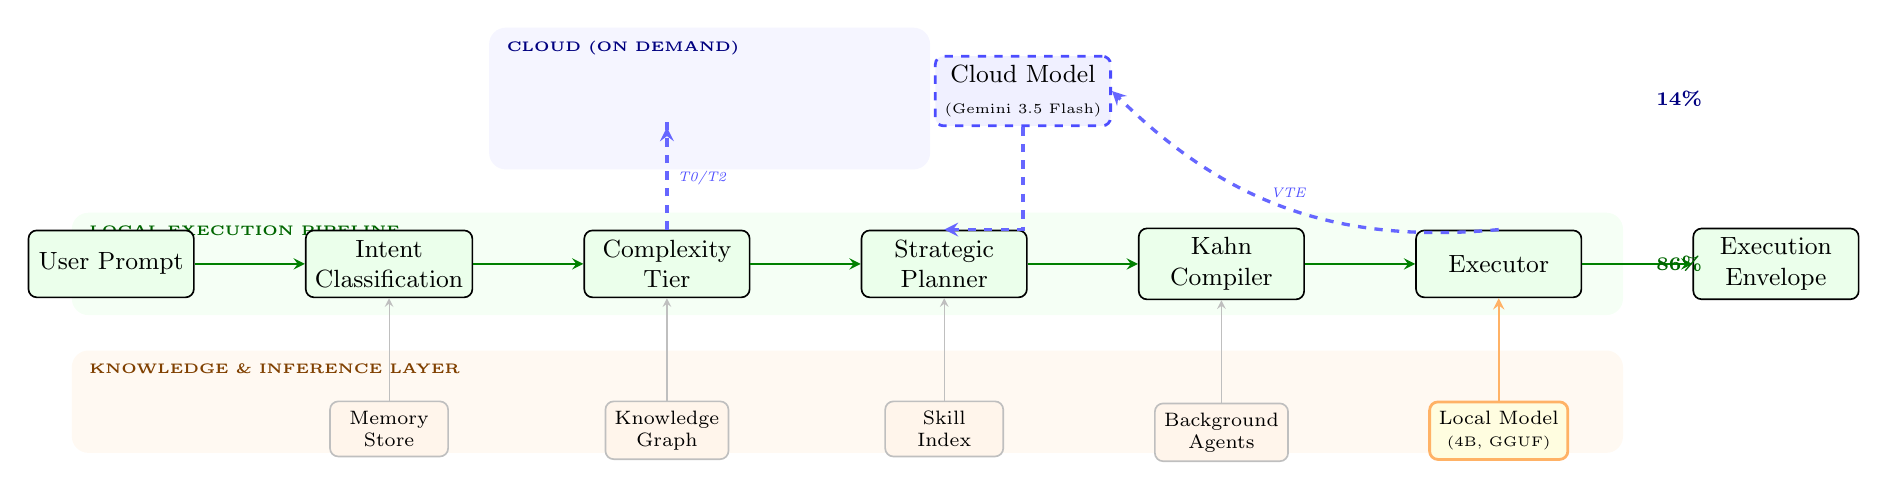
\begin{tikzpicture}[
  node distance=1.0cm and 1.4cm,
  box/.style={draw, rounded corners=3pt, minimum height=0.85cm, minimum width=2.1cm, font=\small, fill=white, align=center, line width=0.6pt},
  cloud/.style={box, draw=blue!70, fill=blue!6, line width=1pt, dashed},
  side/.style={box, draw=gray!50, fill=gray!5, font=\scriptsize, minimum width=1.5cm, minimum height=0.7cm},
  arr/.style={->, >=stealth, thick},
  darr/.style={->, >=stealth, thick, dashed, blue!60},
  region/.style={draw=none, rounded corners=6pt, inner sep=8pt},
]
% Background regions
\fill[green!4, rounded corners=6pt] (-0.5,-0.65) rectangle (19.2,0.65);
\node[font=\tiny\bfseries, green!40!black, anchor=north west] at (-0.4,0.6) {LOCAL EXECUTION PIPELINE};

\fill[orange!5, rounded corners=6pt] (-0.5,-2.4) rectangle (19.2,-1.1);
\node[font=\tiny\bfseries, orange!50!black, anchor=north west] at (-0.4,-1.15) {KNOWLEDGE \& INFERENCE LAYER};

\fill[blue!4, rounded corners=6pt] (4.8,1.2) rectangle (10.4,3.0);
\node[font=\tiny\bfseries, blue!50!black, anchor=north west] at (4.9,2.95) {CLOUD (ON DEMAND)};

% Main pipeline
\node[box, fill=green!8] (prompt) {User Prompt};
\node[box, fill=green!8, right=of prompt] (intent) {Intent\\Classification};
\node[box, fill=green!8, right=of intent] (tier) {Complexity\\Tier};
\node[box, fill=green!8, right=of tier] (planner) {Strategic\\Planner};
\node[box, fill=green!8, right=of planner] (kahn) {Kahn\\Compiler};
\node[box, fill=green!8, right=of kahn] (executor) {Executor};
\node[box, fill=green!8, right=of executor] (envelope) {Execution\\Envelope};

% Cloud
\node[cloud, above=1.3cm of planner, xshift=1.0cm] (cloud) {Cloud Model\\{\tiny (Gemini 3.5 Flash)}};

% Side channels
\node[side, fill=orange!8, below=1.3cm of intent] (memory) {Memory\\Store};
\node[side, fill=orange!8, below=1.3cm of tier] (kg) {Knowledge\\Graph};
\node[side, fill=orange!8, below=1.3cm of planner] (skills) {Skill\\Index};
\node[side, fill=orange!8, below=1.3cm of kahn] (agents) {Background\\Agents};
\node[side, fill=yellow!12, below=1.3cm of executor, line width=1pt, draw=orange!60] (local) {Local Model\\{\tiny (4B, GGUF)}};

% Main flow
\draw[arr, green!50!black] (prompt) -- (intent);
\draw[arr, green!50!black] (intent) -- (tier);
\draw[arr, green!50!black] (tier) -- (planner);
\draw[arr, green!50!black] (planner) -- (kahn);
\draw[arr, green!50!black] (kahn) -- (executor);
\draw[arr, green!50!black] (executor) -- (envelope);

% Cloud escalation
\draw[darr, line width=1.2pt] (tier.north) -- node[right, font=\tiny\itshape, blue!70]{T0/T2} (tier.north |- cloud.south) -- (cloud.south -| tier.north);
\draw[darr, line width=1.2pt] (cloud.south) -- (cloud.south |- planner.north) -- (planner.north);
\draw[darr, line width=1.2pt] (executor.north) to[bend left=25] node[above, font=\tiny\itshape, blue!70]{VTE} (cloud.east);

% Side channel connections
\draw[arr, gray!50, thin] (memory) -- (intent);
\draw[arr, gray!50, thin] (kg) -- (tier);
\draw[arr, gray!50, thin] (skills) -- (planner);
\draw[arr, gray!50, thin] (agents) -- (kahn);
\draw[arr, orange!60, thick] (local) -- (executor);

% Percentage annotation
\node[font=\scriptsize\bfseries, green!40!black, anchor=west] at (19.5, 0) {86\%};
\node[font=\scriptsize\bfseries, blue!50!black, anchor=west] at (19.5, 2.1) {14\%};
\end{tikzpicture}%
}
\caption{\textsc{tzro} system architecture. The green region shows the local execution pipeline (86\% of inference calls). The blue region shows cloud model involvement, used only for T0/T2 planning and Verified Task Execution (14\% of calls). The orange layer provides knowledge and inference services to the pipeline.}
\label{fig:architecture}
\end{figure}

\subsection{Task Lifecycle}

A task proceeds through five stages:

\begin{enumerate}[leftmargin=*]
\item \textbf{Classification}: The Local Model classifies the prompt's intent and Complexity Tier (Section~\ref{sec:complexity_tier}). A complexity gate promotes conversational-sounding prompts to tasks when multi-tool orchestration is required.
\item \textbf{Planning}: The Strategic Planner produces an Abstract Graph. For T1 tasks, the Local Model selects and mutates a Plan Template (Section~\ref{sec:plan_templates}). For T2 tasks, the Cloud Model generates the graph from scratch.
\item \textbf{Compilation}: The Kahn Compiler topologically sorts the Abstract Graph and uses the Strategy Registry to inject infrastructure nodes---Recall Nodes, Semantic Validators, Synthesis Nodes---producing the final Execution DAG (Section~\ref{sec:kahn_compiler}).
\item \textbf{Execution}: The Executor runs nodes in parallel layers, checkpointing completed nodes to SQLite. Each node dispatches to its registered Node Strategy. Edge Thoughts evaluate confidence at each graph traversal.
\item \textbf{Verification}: The Verified Task Execution pipeline (Section~\ref{sec:verified_execution}) applies structural pre-checks, pre-flight validation, and optional cloud verification before returning the Execution Envelope to the consumer.
\end{enumerate}

\subsection{Node Strategy Architecture}

The Executor has \emph{zero} hardcoded knowledge of node types.
All node-type-specific behavior lives in the Strategy Registry, where each strategy declares:
a type identifier,
an execution method (imperative \texttt{Execute} or declarative Stage Plan),
an Edge Thought policy,
a planner reference card (injected into the Strategic Planner's context so it knows what node types exist),
compilation rules (how the Kahn Compiler should augment the node), and
a context role (how the node's output contributes to accumulated context).

Built-in strategies include: \texttt{probe} and \texttt{analyze} (Section~\ref{sec:bounded_exploration}), \texttt{recall} (Section~\ref{sec:recall_node}), \texttt{synthesis}, \texttt{semantic\_validator}, \texttt{branch}, and \texttt{action}.
Custom strategies can be installed via Agent Apps, making the execution model extensible without modifying the core.

\subsection{Domain Language}

\textsc{tzro} maintains a formal vocabulary of $\sim$120 terms with explicit \emph{anti-terms} (e.g., ``Avoid: pipeline, automation track'' for the Kahn Compiler entry).
Anti-terms serve two purposes: they prevent architectural drift by banning synonyms that carry incorrect connotations, and they function as onboarding documentation for both human and AI contributors.
The full glossary is provided in Appendix~\ref{app:glossary}.

% ============================================================================
\section{Durable DAG Compilation}
\label{sec:dag_compilation}
% ============================================================================

\subsection{The Kahn Compiler}
\label{sec:kahn_compiler}

The Kahn Compiler~\cite{kahn1962} takes an Abstract Graph (nodes and edges with sequential dependencies) and produces an Execution DAG through topological sorting.
Nodes with no mutual dependencies are grouped into parallel execution layers.
The compiler then consults the Strategy Registry to inject infrastructure nodes: Recall Nodes downstream of Probe Nodes, Semantic Validators after Action Nodes, and Synthesis Nodes at the terminal position.

The compilation is deterministic: the same Abstract Graph always produces the same Execution DAG.
This property is essential for debugging---a failing benchmark task produces an identical execution plan on every re-run, isolating the problem to execution rather than compilation.

\subsection{Plan Template Registry}
\label{sec:plan_templates}

The Strategic Planner uses an edit-not-create model for T1 tasks.
A GBNF-constrained classification selects one of 7 structural templates (\texttt{explore-only}, \texttt{docgen}, \texttt{research}, \texttt{data-analysis}, \texttt{multi-probe-synthesis}, \texttt{codegen}, \texttt{action-chain}), and the Local Model mutates the template to fit the specific task.
The model has full mutation authority---it can add, remove, or modify nodes, edges, tools, and configuration---but starts from a structurally sound scaffold rather than generating from scratch.

This design was motivated by benchmark analysis showing that the 4B model generates structurally inconsistent DAGs when planning from scratch, because simultaneously designing a graph and serializing it to JSON exceeds the model's effective reasoning capacity.
The template reduces the cognitive burden to ``edit and serialize'' rather than ``design and serialize.''
Existing validation (\texttt{findInvalidTools}, \texttt{CompileAndSort}, \texttt{repairGraphWithProbe}, cloud escalation) catches any structural errors post-mutation.

\subsection{Durable Checkpointing}

All state is persisted to SQLite at node boundaries.
Completed node outputs are committed before execution of dependent nodes begins.
If the process crashes mid-task, restarting picks up from the last completed node---no re-execution of already-finished work.

Within Probe Nodes, checkpointing operates at finer granularity: each Thought Chain step is committed individually, and the Phase Runner persists completed phases to the \texttt{phase\_results} table.
This two-level durability means a crash at step 15 of a 20-step probe resumes from step 15, not from the beginning of the probe.

\subsection{Dynamic Graph Mutation}

While the parent DAG is static, limited runtime mutation is supported through two mechanisms:
(1) the Hybrid Branch Evaluator, which uses JSONPath matching (with semantic LLM fallback) to evaluate conditional edges;
and (2) Edge Thought--driven node spawning, where low-confidence edge traversals can trigger additional exploration nodes.
A mutation budget constrains the total number of runtime-added nodes to prevent unbounded graph growth.

% ============================================================================
\section{Local-First Cost Arbitrage}
\label{sec:cost_arbitrage}
% ============================================================================

The central economic claim of \textsc{tzro} is that most agentic execution is \emph{routing}---deciding which tool to call, which file to read, which parameter to extract---not \emph{reasoning}---deciding what code to write, what architecture to choose, what tradeoffs to make.
Routing is a classification problem that a 4B model handles reliably; reasoning is a generation problem that benefits from frontier model capacity.
This section formalizes that distinction through two complementary routing mechanisms and a self-improving correction pipeline.

% ---------------------------------------------------------------------------
\subsection{The Routing Hypothesis}
\label{sec:routing_hypothesis}

We define a \emph{routing decision} as one where the correct action can be determined from the available context (accumulated node outputs, tool schemas, task goal) without requiring world knowledge or complex multi-constraint reasoning.
Examples include: selecting \texttt{read\_file} when an exploration plan calls for reading a specific path; extracting a \texttt{query} parameter from a natural language question and a database schema; choosing between \texttt{web\_search} and \texttt{web\_browse} based on whether a URL is already known.

We define a \emph{reasoning decision} as one where the correct action requires synthesis, judgment, or knowledge beyond the immediate context.
Examples include: generating architecturally sound code; evaluating whether a synthesis is factually complete; planning a multi-step workflow from an ambiguous natural language prompt.

Analysis of the benchmark data (Section~\ref{sec:eval_cost}) confirms this split empirically: in Run 28, 86\% of inference calls (412 of 479) were handled locally.
The 67 cloud inference calls were concentrated in three categories: task-level planning (Complexity Tier T2), terminal output verification (Verified Task Execution), and parameter extraction failures (Confidence Tier escalation).

% ---------------------------------------------------------------------------
\subsection{Complexity Tier: Task-Level Routing}
\label{sec:complexity_tier}

At task intake, the Local Model classifies each prompt into one of three Complexity Tiers:

\begin{itemize}[leftmargin=*]
\item \textbf{T0 Direct}: Conversational Q\&A requiring world knowledge or low latency. Routed directly to the Cloud Model for a streamed response. No DAG compilation.
\item \textbf{T1 Planned}: Structured multi-step work. The Local Model selects a Plan Template via GBNF-constrained classification, mutates it to fit the specific task, and executes all nodes locally.
\item \textbf{T2 Supervised}: Complex architectural judgment. The Cloud Model generates the Abstract Graph from scratch (no template constraint), the Kahn Compiler compiles it, and the Local Model executes the resulting nodes.
\end{itemize}

A complexity gate detects prompts that \emph{sound} conversational but actually require multi-tool orchestration (e.g., ``can you explain how the cache works?'' for a codebase with a complex cache implementation). When classification resolves to T1 or T2 despite a conversational surface form, the system promotes the prompt to a task and notifies the user.

The key architectural decision was that Complexity Tier routing is \emph{non-exclusive}: it determines who \emph{plans}, not who \emph{executes}.
T2 tasks use the cloud for planning but the local model for execution, keeping per-node inference costs at zero while leveraging frontier reasoning for graph design.

% ---------------------------------------------------------------------------
\subsection{Confidence Tier: Per-Node Routing}
\label{sec:confidence_tier}

Within a task, individual DAG nodes face a second routing decision.
Before each action node's GBNF-constrained parameter extraction, the Local Model runs a \emph{Confidence Tier pre-flight}: a self-assessment asking whether it can extract the required parameters from the accumulated context and tool schema.

\begin{itemize}[leftmargin=*]
\item \textbf{Sufficient}: The Local Model proceeds with parameter extraction and tool dispatch.
\item \textbf{Insufficient}: The node escalates to the Cloud Model, which re-runs the extraction. If the Cloud Model succeeds, a Corrective Micro-Skill is extracted (Section~\ref{sec:corrective_skills}).
\end{itemize}

The Confidence Tier is deliberately scoped to \emph{parameter extraction only}.
Terminal output quality---whether the final synthesis is factually correct, well-organized, and complete---is owned by the Verification Gate (Section~\ref{sec:verified_execution}).
This separation prevents the pre-flight from becoming a general-purpose quality gate, which would route too many nodes to the cloud and undermine cost arbitrage.

A sticky escalation threshold (default: 3 consecutive \texttt{insufficient} results) forces cloud routing for the remainder of the task, preventing the system from repeatedly attempting local extraction on a task that has exceeded the model's capabilities.

% ---------------------------------------------------------------------------
\subsection{Corrective Micro-Skills}
\label{sec:corrective_skills}

When the Local Model claims \texttt{sufficient} confidence but the subsequent tool call fails, the node surgically escalates to the Cloud Model.
If the Cloud Model succeeds, the system immediately extracts a \emph{Corrective Micro-Skill} from the diff between the failed local output and the successful cloud output.

Corrective Micro-Skills are anti-pattern SOPs: structured Markdown documents describing the specific failure pattern and its correction (e.g., ``use double quotes for SOQL string values,'' ``include the \texttt{WHERE} clause before \texttt{GROUP BY}'' for a particular API).
They are persisted via the existing \texttt{synthesized\_skills} pipeline and injected into the Local Model's context on future invocations matching the same trigger.

This design was chosen over historical success-rate injection, where per-tool success/failure ratios would be injected into the classification prompt.
Success rates are a blunt instrument: a high-frequency tool with a specific failure pattern would be over-penalized and broadly routed to the cloud, contradicting the goal of maximizing local execution.
Corrective Micro-Skills are surgical---they fix the specific anti-pattern while keeping the tool routed locally for everything else.

The result is a system that self-improves without weight updates: each cloud escalation teaches the local model to avoid one more failure pattern, progressively reducing the escalation rate over time.

% ---------------------------------------------------------------------------
\subsection{Task Sizing as a Design Principle}
\label{sec:task_sizing}

The apparent ``limitations'' of 4B models are often symptoms of improper task decomposition by the orchestration harness rather than fundamental capability gaps.
The analogy is staffing: you assign an intern appropriately-scoped tasks, not entire features.
The harness bears the same responsibility.

When work is decomposed into properly-scoped units:
\begin{itemize}[leftmargin=*]
\item The local model handles the full execution pipeline reliably, because each unit requires routing (tool selection, parameter extraction) rather than open-ended reasoning.
\item Long coherent generation ($>$500 tokens) becomes unnecessary, because outputs are naturally bounded by the unit of work.
\item Complex multi-constraint decisions decompose into sequential, manageable steps, each within the model's effective attention window.
\end{itemize}

The \emph{remaining} genuine limitations---world knowledge gaps, novel API integration without micro-skills, complex architectural judgment---are precisely the cases handled by Complexity Tier routing (T0/T2) and Confidence Tier escalation.
The local model's boundary is not a hard capability wall but a soft decomposition threshold: with proper sizing, it moves outward; without it, even frontier models struggle.

% ---------------------------------------------------------------------------
\subsection{Cost Analysis}
\label{sec:cost_numbers}

Table~\ref{tab:cost_analysis} in Section~\ref{sec:eval_cost} presents the full cost breakdown for Run 28.
The headline numbers: 25 tasks, \$2.57 total cost, 1.66M local tokens consumed at zero marginal cost, 243K cloud tokens at \$0.10/task average.
The cloud-to-local inference ratio of 1:6.1 confirms that the routing hypothesis holds in practice---for every cloud inference call, the system makes 6.1 local calls that would have cost approximately \$0.01--0.03 each on a frontier API.

At scale, the cost arbitrage compounds.
A developer running 50 tasks per day would spend approximately \$5/day in cloud costs while consuming roughly 3.3M local tokens---equivalent to approximately \$33--66 in frontier API costs, depending on the provider---at zero additional expense.

% ============================================================================
\section{Bounded Autonomous Exploration}
\label{sec:bounded_exploration}
% ============================================================================

Codebase exploration, web research, and data analysis are \emph{dynamically shaped}: the planner cannot predict directory structures, file counts, search result quality, or database schemas at planning time.
A static DAG requires the graph shape to be known before execution begins.
This section describes how \textsc{tzro} reconciles autonomous exploration with deterministic DAG execution through Probe Nodes, a three-pass Thought Chain, structured Phase Runners, and content-aware Recall.

% ---------------------------------------------------------------------------
\subsection{Probe Nodes}
\label{sec:probe_nodes}

The Probe Node resolves the tension between exploration and determinism.
From the parent DAG's perspective, it is an opaque node: one input (a natural language goal), one output (a terminal synthesis).
The parent DAG stays static, acyclic, and checkpointable.
Internally, the Probe Node runs a bounded multi-step exploration loop with three key constraints:

\begin{enumerate}[leftmargin=*]
\item \textbf{Step budget}: A configurable maximum (default 20) that guarantees termination regardless of model behavior.
\item \textbf{Scoped tool list}: Each Probe Node declares its \texttt{allowedTools}---typically \texttt{read\_file}, \texttt{list\_dir}, \texttt{search\_files} for codebase exploration, or \texttt{web\_search}, \texttt{web\_browse} for web research.
Tools outside the allowed set cannot be called.
\item \textbf{Convergence detection}: The model can signal early termination when it judges exploration complete, subject to a Synthesis Validation Gate (Section~\ref{sec:synthesis_gate}).
\end{enumerate}

Three alternative designs were evaluated and rejected:
\emph{Scatter Nodes} (runtime DAG expansion) would introduce graph mutation to the executor, violating the static DAG invariant.
\emph{Smart planning} (the cloud model predicts project structure) assumes knowledge of arbitrary filesystems---untenable for unfamiliar codebases.
\emph{A separate ReAct agent loop} would create a second execution mode that would eventually absorb all work, causing the DAG mode to atrophy.
The Probe Node avoids all three by containing autonomy \emph{inside} a DAG node rather than replacing the DAG.

% ---------------------------------------------------------------------------
\subsection{Three-Pass Thought Chain}
\label{sec:thought_chain}

Each step of the Thought Chain executes three inference passes, each targeting a specific model via the \texttt{ModelTarget} routing enum (\texttt{TargetWorker} for the 4B model, \texttt{TargetRouter} for the 1B model):

\paragraph{Pass 1: Worker (unconstrained reasoning).}
The 4B Worker model sees four inputs: (1) the probe goal, (2) semantically retrieved prior thoughts (top-$K$ via ONNX embedding cosine similarity over persisted thought entries), (3) the current step's task, and (4) the previous tool output (bounded).
It produces free-text reasoning with optional \texttt{<ACTION>} tag hints.
Critically, it does \emph{not} see the full exploration history---only the latest tool output and retrieved thoughts---which bounds context pressure regardless of exploration depth.

\paragraph{Pass 2: Router (GBNF-constrained extraction).}
The 1B Router model extracts a structured action from the Worker's reasoning using a GBNF grammar that constrains output to: \texttt{\{action: "tool\_call" | "synthesize", tool: string, arguments: object\}}.
This pass \emph{always runs}---it is the designed extraction path, not a fallback.
When the Worker's reasoning contains complete \texttt{<ACTION>} tags (approximately 10\% of cases), the Router receives targeted extraction context.
Otherwise, it receives the full reasoning output.

This two-pass design replaced a single-pass approach where the Worker was expected to emit both reasoning and structured tool calls.
The single-pass approach failed approximately 90\% of the time, requiring a rescue fallback with a 1500-character truncated context window.
The two-pass design achieves near-100\% extraction reliability by separating the cognitive tasks: the Worker \emph{reasons}, the Router \emph{structures}.

\paragraph{Pass 3: Synthesis Validation Gate.}
\label{sec:synthesis_gate}
When the Router signals \texttt{synthesize}, the Probe does not immediately terminate.
Instead, a third pass sends the Worker a validation prompt containing: the current step position within the budget, the number of successful tool calls, and the list of unused tools.
The Worker returns a structured judgment: \texttt{\{ready: bool, reason: string, additionalSteps: int\}}.
If the Worker returns \texttt{ready: false}, the synthesis is rejected (up to 2 rejections), the step budget is extended, and exploration continues.

This gate was introduced because the 1B Router consistently signaled premature synthesis---as early as step 8 of 20---because it cannot judge information completeness.
The Worker's larger context window and reasoning capacity make it a more reliable arbiter of exploration sufficiency.

\paragraph{Durability.}
Each thought step is committed to SQLite immediately upon completion.
If the process crashes at step 12, it resumes from the last committed thought plus the rolling compaction summary.
Rolling compaction merges every 3 thoughts into a running text summary, serving both as a context-efficient history representation and a crash-recovery checkpoint.

Figure~\ref{fig:thought_chain} illustrates the three-pass structure.

\begin{figure}[t]
\centering
\resizebox{0.92\textwidth}{!}{%
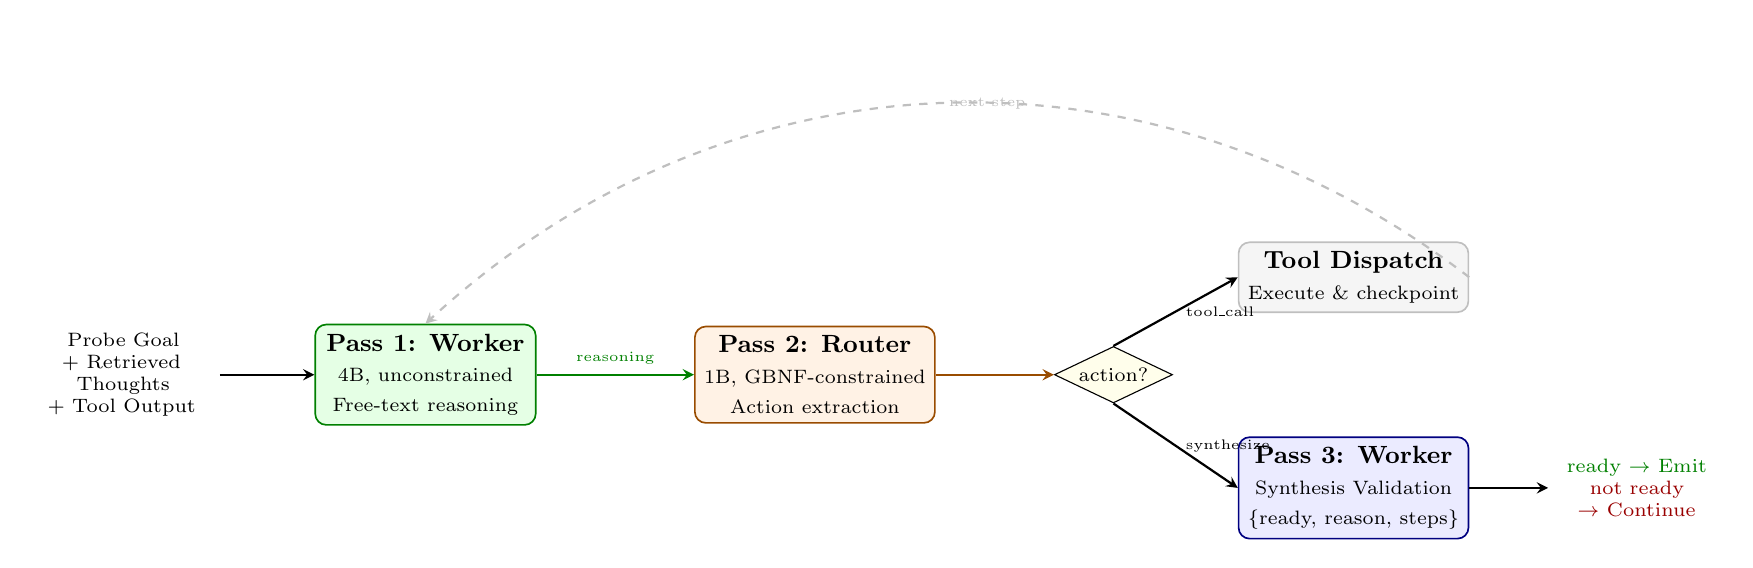
\begin{tikzpicture}[
  node distance=0.8cm and 1.8cm,
  pass/.style={draw, rounded corners=4pt, minimum height=1.2cm, minimum width=2.8cm, font=\small, align=center, line width=0.6pt},
  input/.style={font=\scriptsize, align=center, text width=2.2cm},
  arr/.style={->, >=stealth, thick},
  lbl/.style={font=\tiny, midway, above},
]
% Pass 1
\node[pass, fill=green!10, draw=green!50!black] (p1) {\textbf{Pass 1: Worker}\\{\scriptsize 4B, unconstrained}\\{\scriptsize Free-text reasoning}};
\node[input, left=1.2cm of p1] (p1in) {Probe Goal\\+ Retrieved Thoughts\\+ Tool Output};
\draw[arr] (p1in) -- (p1);

% Pass 2
\node[pass, fill=orange!10, draw=orange!60!black, right=2.0cm of p1] (p2) {\textbf{Pass 2: Router}\\{\scriptsize 1B, GBNF-constrained}\\{\scriptsize Action extraction}};
\draw[arr, green!50!black] (p1) -- node[lbl]{reasoning} (p2);

% Decision
\node[draw, diamond, aspect=2, right=1.5cm of p2, minimum width=1.5cm, font=\scriptsize, fill=yellow!8, inner sep=1pt] (dec) {action?};
\draw[arr, orange!60!black] (p2) -- (dec);

% Tool call path
\node[pass, fill=gray!8, draw=gray!50, above right=0.6cm and 1.2cm of dec, minimum height=0.8cm, minimum width=2.0cm] (tool) {\textbf{Tool Dispatch}\\{\scriptsize Execute \& checkpoint}};
\draw[arr] (dec.north) -- node[right, font=\tiny]{tool\_call} (tool.west);

% Synthesize path -> Pass 3
\node[pass, fill=blue!8, draw=blue!50!black, below right=0.6cm and 1.2cm of dec, minimum height=1.0cm] (p3) {\textbf{Pass 3: Worker}\\{\scriptsize Synthesis Validation}\\{\scriptsize \{ready, reason, steps\}}};
\draw[arr] (dec.south) -- node[right, font=\tiny]{synthesize} (p3.west);

% Pass 3 outputs
\node[font=\scriptsize, right=1.0cm of p3, text width=2cm, align=center] (out) {\textcolor{green!50!black}{ready $\to$ Emit}\\\textcolor{red!60!black}{not ready $\to$ Continue}};
\draw[arr] (p3) -- (out);

% Loop back
\draw[arr, gray!50, dashed] (tool.east) to[bend right=40] node[right, font=\tiny]{next step} (p1.north);
\end{tikzpicture}%
}
\caption{Three-Pass Thought Chain within a Probe Node. Pass~1 (Worker, 4B) produces unconstrained reasoning. Pass~2 (Router, 1B) extracts a structured action via GBNF grammar. On \texttt{synthesize}, Pass~3 (Worker) validates completeness before allowing early termination. The separation of reasoning from structure extraction is the key reliability insight: the single-pass approach failed $\sim$90\% of the time.}
\label{fig:thought_chain}
\end{figure}

% ---------------------------------------------------------------------------
\subsection{Phase Runner}
\label{sec:phase_runner}

The flat Thought Chain described above has a fundamental limitation: it provides no structural guidance for multi-phase tasks.
A research task, for example, requires distinct phases (searching, evaluating sources, deep reading, cross-referencing, synthesizing) that benefit from different tool sets and step budgets.
Under the flat loop, the 4B model consistently hit a quality ceiling around 2.5/5.0 on research tasks because it would search, read one result, and immediately attempt synthesis.

The Phase Runner is a state machine that replaces the flat loop with a structured pipeline of \emph{Phases}.
Each Phase declares:

\begin{itemize}[leftmargin=*]
\item \textbf{Scoped tools}: A Phase restricts the available tools.
The Search phase of a research pipeline only exposes \texttt{web\_search}; the Deep-Read phase only exposes \texttt{web\_browse}.
This prevents premature synthesis and tool misuse.
\item \textbf{Step budget}: Per-phase budgets (typically 2--8 steps) enforce deterministic termination at each stage, replacing the single global 20-step budget.
\item \textbf{Model target}: Per-phase routing to the Router or Worker, allowing lightweight phases to use the faster 1B model.
\item \textbf{Recovery strategy}: Per-phase \texttt{OnExhaustion} behavior---\texttt{retry}, \texttt{skip}, \texttt{fail}, or \texttt{backtrack} (re-enter an earlier phase with accumulated context).
\end{itemize}

Three node-type-specific pipelines are built via closures that wire domain-specific \texttt{ToolFixup} and \texttt{ToolPostProcess} hooks:

\begin{itemize}[leftmargin=*]
\item \textbf{Probe}: Orient $\to$ Discover $\to$ Deep-Read $\to$ Synthesize.
Used for codebase exploration---Orient identifies the project structure, Discover navigates to key files, Deep-Read extracts details, Synthesize produces the terminal output.
\item \textbf{Analyze}: Schema-Orient $\to$ Query-Dev $\to$ Compute $\to$ Synthesize.
Used for data analysis---Schema-Orient inspects the cached data schema, Query-Dev constructs SQL, Compute executes queries, Synthesize interprets results.
Structural gates enforce ordering: \texttt{introspect\_cache} must be called before Query-Dev can begin; at least 2 analytical queries must execute before Compute concludes.
\item \textbf{Research}: Search $\to$ Rank $\to$ Deep-Read $\to$ Cross-Ref $\to$ Synthesize.
Used for web research---the 5-phase structure forces the model through disciplined source evaluation rather than single-source synthesis.
\end{itemize}

The Phase Runner persists completed phases to the \texttt{phase\_results} database table for durable resume and produces a Phase Manifest containing per-phase metadata (steps used, tools called, backtracks) for observability and skill extraction.

\paragraph{Tool hooks.}
The Phase Runner core remains deliberately simple---it dispatches tools and manages transitions.
All node-type-specific intelligence lives in two hook functions:
\texttt{ToolFixup} repairs arguments before dispatch (e.g., extracting SQL from reasoning text when the model writes a query in prose but fails to emit it as a parameter), and
\texttt{ToolPostProcess} tracks state after dispatch (e.g., marking URLs as visited, capturing analytical evidence).
These hooks are wired per-node-type via builder closures, keeping the Phase Runner generic.

% ---------------------------------------------------------------------------
\subsection{Substrate Mode Classification}
\label{sec:substrate_mode}

Not all probe tasks require a multi-step Thought Chain.
Before entering the exploration loop, a keyword-based classifier routes probes to one of four substrate modes:

\begin{enumerate}[leftmargin=*]
\item \textbf{Overview}: Tasks requesting high-level summaries (``explain the architecture,'' ``list the main modules'').
Resolved via \emph{Directory Manifest}---a recursive tree-sitter symbol extraction with doc comment previews---fed directly into a single-shot \emph{Direct Synthesis} inference call.
No Thought Chain, no tool calls.

\item \textbf{Focused}: Tasks targeting specific components (``explain the cache invalidation logic'').
Uses a \emph{Call Graph Index} to identify entry points, then navigates via entry-point traversal with \emph{Graph-Driven Context} assembly.

\item \textbf{Aggregate}: Tasks requiring content processing across many files (``generate a comprehensive README'').
Uses \emph{MapReduceSynthesis}: content is chunked, each chunk is summarized in parallel (the ``map'' calls), and a final ``reduce'' call synthesizes the summaries.
This replaces $N \times 10$ Thought Chain steps with $N + 1$ inference calls.
A single-chunk passthrough avoids unnecessary overhead when content fits the context window.

\item \textbf{Unknown}: Goals that don't match any keyword pattern fall through to the standard Thought Chain or Phase Runner.
This is the safe default---the classifier never blocks a probe from running.
\end{enumerate}

This pre-routing eliminated unnecessary Thought Chain loops for tasks where pre-computed context plus single-shot synthesis produces equivalent or better results in a fraction of the time (1 inference call vs.\ 10--15).

% ---------------------------------------------------------------------------
\subsection{Recall Node and Refinement Pass}
\label{sec:recall_node}

The Recall Node sits downstream of Probe Nodes in the DAG and is responsible for assembling a coherent synthesis from one or more Probe outputs.
Its design went through a critical architectural inversion during the evaluation period (Section~\ref{sec:eval_quality_arc}, the August 4 regression).

\paragraph{The Synthesis Cliff.}
The original Recall Node attempted to process raw Thought Chain history---the complete sequence of tool outputs, reasoning, and intermediate synthesis---in a single inference call.
This approach produced coherent output for short probes (5--8 steps) but hit a ``Synthesis Cliff'' at scale: probes with 15+ steps generated 69K--99K character contexts that overwhelmed the model, producing incoherent or truncated synthesis.

\paragraph{Recall Loop Inversion.}
The redesigned Recall Node inverts the execution contract from ``agentic discovery'' to ``deterministic floor + Refinement Pass'':

\begin{enumerate}[leftmargin=*]
\item \textbf{Deterministic compaction} builds a baseline \texttt{refinedContext} from all upstream Thought Chain steps before any agentic processing begins.
Each step's tool output is classified and compacted using type-appropriate strategies (Section~\ref{sec:context_management}):
code outputs receive deterministic Code Skeleton extraction;
tabular data receives schema-preserving sample rows;
web and text content receives LLM-driven fact extraction via the 1B Router.

\item \textbf{Refinement Pass} (the agentic loop) receives the pre-built baseline and can selectively fetch full details for steps where the compaction lost important information, adding facts via an \texttt{update\_refined\_context} tool.
In 89\% of observed executions, the model signals immediate readiness---the deterministic baseline is sufficient.
In the remaining 11\%, the model refines the baseline additively.

\item \textbf{Terminal synthesis} produces the final output from the \texttt{refinedContext}, the original goal, and an injected \textbf{Symbol Index}---a deterministic inventory of all public symbols extracted via tree-sitter AST parsing during the Probe's tool calls.
\end{enumerate}

\paragraph{Symbol Anchor Check.}
A post-synthesis verification step diffs the symbols referenced in the synthesis against the Symbol Index.
If more than 20\% of referenced symbols are unanchored (not found in the index, excluding qualified external references like \texttt{context.Context}), a targeted correction pass is triggered.
This mechanism was introduced after docgen benchmarks revealed that cooperative mode produced 67\% hallucinated type names---a defect masked by LLM-as-judge scoring, which rewarded structural formatting without verifying factual accuracy (the cloud judge scored 4.25/5.0; cross-verification by the local 4B model scored 2.65/5.0, exposing a 38\% inter-rater inflation gap).

% ---------------------------------------------------------------------------
\subsection{Lessons Learned}
\label{sec:exploration_lessons}

Three key findings emerged from the evolution of the exploration pipeline:

\paragraph{Flat loops hit an attention ceiling.}
The flat Thought Chain consistently degraded after step 8--10, with the model losing track of its exploration plan and repeating tool calls or entering futile loops.
The Phase Runner's per-phase scoping directly addresses this: each phase starts with a fresh context injection, and the small per-phase budgets (2--8 steps) keep the model within its effective attention window.

\paragraph{Separation of reasoning and structure is essential.}
Every attempt to have the 4B model produce both free-text reasoning \emph{and} structured tool calls in a single inference pass failed at scale ($\sim$90\% failure rate on action tag emission).
The two-pass design (Worker reasons, Router structures) achieves near-100\% reliability by decomposing a hard multi-objective generation task into two easy single-objective tasks.

\paragraph{Deterministic floors outperform agentic discovery.}
The Recall Loop Inversion demonstrated a counterintuitive finding: building a deterministic baseline via content-aware compaction and then \emph{optionally} refining it agentically produces better results than asking the model to discover what's important from scratch.
The 89\% immediate-ready rate suggests that the deterministic compaction captures the vast majority of relevant information---the agentic loop's marginal contribution is real but small.

% ============================================================================
\section{Content-Aware Context Management}
\label{sec:context_management}
% ============================================================================

LLM context windows are finite, and attention quality degrades with length.
Tool outputs are heterogeneous---JSON, HTML, source code, tabular data, raw text---and treating them uniformly wastes context capacity on low-information content.

\subsection{Compaction Pipeline}

Raw tool outputs pass through a 5-layer pre-processing pipeline (JSON flattening, HTML stripping, base64 removal, whitespace normalization, length capping) before entering the Structured Compactor.
The Compactor classifies each output segment and applies type-appropriate strategies:

\begin{itemize}[leftmargin=*]
\item \textbf{Code} (\texttt{SegmentCode}): Deterministic Code Skeleton extraction---function signatures, type declarations, and comments are preserved; function bodies are replaced with fingerprints (\texttt{// [body: 42 lines, calls: foo(), bar()]}).
Code is \emph{never} LLM-compressed.
The rationale: well-written code (both human and agent-authored) carries extensive inline comments and doc comments that explain functionality.
The signatures and comments preserve understanding without the raw logic.
\item \textbf{Reasoning text} (\texttt{SegmentText}, from model output): The 1B Router extracts key conclusions per 500-character chunk, preserving the model's \emph{decisions} while stripping its \emph{deliberation}.
\item \textbf{Web/text content}: Fact extraction via the Router (``Extract all factual claims, statistics, names, comparisons, and URLs as a bulleted list''), achieving approximately 4:1 compression while preserving information density.
\item \textbf{Tabular data} (\texttt{SegmentTabular}): Schema-preserving sample rows for the context envelope, plus materialization into the \textbf{SQL Cache Store}---ephemeral SQLite tables that enable downstream Analyze Nodes to run actual SQL queries against the data rather than parsing raw text.
\end{itemize}

\subsection{Accumulated Context Budgeting}

The Accumulated Context assembles outputs from completed nodes into the prompt for downstream nodes.
A budgeting system controls context size through three mechanisms:
per-node-type weight budgets (Probe output receives more budget than Action output),
node count windowing (only the $N$ most recent nodes of each type are included), and
content-aware per-node truncation via the Structured Compactor.

\subsection{Binding Resolution}

Dynamic bindings (\texttt{\{\{nodes.probe\_1.output.summary\}\}}) are resolved through a 5-tier Response Resolver cascade that normalizes heterogeneous tool outputs into resolvable property maps.
Critically, the \emph{Proactive Binding Splice} strips deterministically-resolved values from the tool schema before inference and splices them back after inference.
The model never sees or generates these parameters---it cannot get them wrong.
This mechanism eliminated 57\% of GBNF parameter failures in benchmark analysis by removing the model from the path entirely for known values.

\subsection{Generation Guard}

A multi-tier degeneration detection system monitors inference output for quality collapse:
character-level collapse (repeated characters or tokens),
block-level repetition (n-gram analysis with length-scaled thresholds),
and compression-ratio analysis (zlib ratio indicating low-information content).
Thresholds are content-mode-aware---code outputs tolerate more structural repetition than prose.
For streaming backends, detection triggers immediate abort; for non-streaming backends, degenerate tails are truncated.

% ============================================================================
\section{Code Generation Quality Gates}
\label{sec:codegen_quality}
% ============================================================================

\textsc{tzro}'s code generation pipeline produces output through a multi-stage quality gate chain:

\begin{enumerate}[leftmargin=*]
\item \textbf{Semantic Validator}: Coerces the model's output from XML-like tags into structured JSON, replacing deep GBNF constraints that slowed inference 2--5$\times$.
\item \textbf{Compilation Gate}: Runs language-specific syntax and compilation verification (\texttt{go build}, \texttt{tsc --noEmit}, etc.) to catch structural errors before human review.
\item \textbf{Spec Compliance Gate}: An LLM-evaluated checklist where each requirement from the original specification is scored as IMPLEMENTED or MISSING, producing a concrete gap analysis.
\item \textbf{Preservation Assertion}: An AST-based diff that detects dropped public symbols---functions, types, methods that existed in the original file but are missing from the generated output. This catches the 4B model's tendency toward catastrophic symbol dropping during full-file generation.
\item \textbf{Tiered escalation}: One local retry with corrective feedback, then cloud escalation if the retry fails.
\end{enumerate}

\subsection{Edit Loop}

For existing files ($\geq$20 lines), \textsc{tzro} uses a hunk-based iterative editing strategy rather than full-file regeneration:

\begin{enumerate}[leftmargin=*]
\item \textbf{Plan step}: The model produces unconstrained prose listing the discrete changes needed.
\item \textbf{Hunk loop}: Each step produces a GBNF-constrained JSON hunk (\texttt{\{searchContent, replaceContent, done\}}) applied via surgical text replacement.
\item \textbf{Budget guard}: Maximum 15 steps; \texttt{done: true} exits early.
\end{enumerate}

This achieves 30--50$\times$ token reduction over full-file generation for files of moderate size, because only the changed regions are generated.
The threshold for entering Edit Loop mode is 20 lines---below that, full-file generation is more efficient.

% ============================================================================
\section{Verified Task Execution}
\label{sec:verified_execution}
% ============================================================================

Verified Task Execution is the final quality gate in the pipeline.
The insight motivating its design: benchmark data showed the 4B model producing 5.0-quality output on some runs and 1.0 on others for the \emph{same task, same model, same framework}.
The capability exists in the weights; the problem is \emph{variance with no verification mechanism}.

\subsection{The Pipeline}

\begin{enumerate}[leftmargin=*]
\item \textbf{Structural Pre-Check} (local, deterministic, $<$1ms): Detects Generation Guard markers, meta-commentary degeneration (``As an AI\ldots'' patterns), and length/truncation anomalies. Rejects obviously degenerate output before cloud verification.
\item \textbf{Pre-Flight Validation} ($<$10ms): Coverage verification via key-term matching against the original goal, and content validation (URL format checking, quote verification).
\item \textbf{Verification Gate} (cloud): Evaluates the terminal synthesis against the original goal and the Recall Node's \texttt{refinedContext}. Returns a Verification Rubric with per-dimension float scores and an accept/reject decision.
\item \textbf{Cloud Re-Synthesis} (if rejected): The \emph{same} cloud call that rejects also produces a re-synthesis from the \texttt{refinedContext}---no additional round-trip. This is a key design decision: combining verification and re-synthesis into a single call saves latency and cost.
\end{enumerate}

The pipeline adds approximately \$0.03--0.05 per Probe/Analyze task in cloud costs.
All nine pre-existing compensatory mechanisms (Generation Guard, DRY sampling, meta-commentary detection, Synthesis Validation Gate, Two-Pass Extraction, Recall Loop Inversion, No-Action Retry, Exploration Queue, SQL Auto-Extraction) are retained---their purpose reframes from ``compensate for bad output'' to ``maximize context quality for higher verification accept rates.''

A \texttt{strict-local} Privacy Level disables cloud verification entirely, running only the Structural Pre-Check. The user accepts the output variance in exchange for complete privacy.

Figure~\ref{fig:vte_pipeline} illustrates the VTE decision flow.

\begin{figure}[t]
\centering
\resizebox{0.88\textwidth}{!}{%
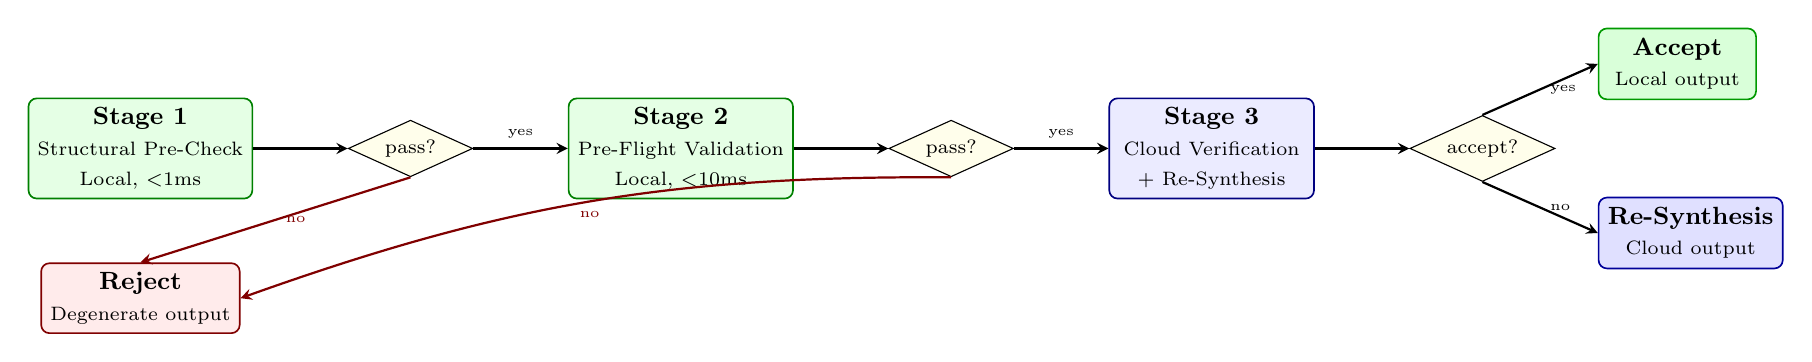
\begin{tikzpicture}[
  node distance=0.9cm and 1.6cm,
  stage/.style={draw, rounded corners=3pt, minimum height=0.9cm, minimum width=2.6cm, font=\small, align=center, line width=0.6pt},
  decision/.style={draw, diamond, aspect=2.2, font=\scriptsize, inner sep=2pt, fill=yellow!8},
  arr/.style={->, >=stealth, thick},
]
% Stages
\node[stage, fill=green!10, draw=green!50!black] (s1) {\textbf{Stage 1}\\{\scriptsize Structural Pre-Check}\\{\scriptsize Local, $<$1ms}};
\node[decision, right=1.2cm of s1] (d1) {pass?};
\draw[arr] (s1) -- (d1);

\node[stage, fill=green!10, draw=green!50!black, right=1.2cm of d1] (s2) {\textbf{Stage 2}\\{\scriptsize Pre-Flight Validation}\\{\scriptsize Local, $<$10ms}};
\draw[arr] (d1) -- node[above, font=\tiny]{yes} (s2);

\node[decision, right=1.2cm of s2] (d2) {pass?};
\draw[arr] (s2) -- (d2);

\node[stage, fill=blue!8, draw=blue!50!black, right=1.2cm of d2] (s3) {\textbf{Stage 3}\\{\scriptsize Cloud Verification}\\{\scriptsize + Re-Synthesis}};
\draw[arr] (d2) -- node[above, font=\tiny]{yes} (s3);

\node[decision, right=1.2cm of s3] (d3) {accept?};
\draw[arr] (s3) -- (d3);

% Accept path
\node[stage, fill=green!15, draw=green!60!black, above right=0.4cm and 1.0cm of d3, minimum width=2.0cm] (accept) {\textbf{Accept}\\{\scriptsize Local output}};
\draw[arr] (d3.north) -- node[right, font=\tiny]{yes} (accept.west);

% Reject path
\node[stage, fill=blue!12, draw=blue!60!black, below right=0.4cm and 1.0cm of d3, minimum width=2.0cm] (resyn) {\textbf{Re-Synthesis}\\{\scriptsize Cloud output}};
\draw[arr] (d3.south) -- node[right, font=\tiny]{no} (resyn.west);

% Reject early paths
\node[stage, fill=red!8, draw=red!50!black, below=0.8cm of s1, minimum width=2.0cm, minimum height=0.7cm] (rej) {\textbf{Reject}\\{\scriptsize Degenerate output}};
\draw[arr, red!50!black] (d1.south) -- node[right, font=\tiny]{no} (rej.north);
\draw[arr, red!50!black] (d2.south) to[bend right=10] node[below, font=\tiny]{no} (rej.east);
\end{tikzpicture}%
}
\caption{Verified Task Execution pipeline. Stages 1--2 are local deterministic checks ($<$10ms total). Stage 3 is a single cloud call that both evaluates quality and produces a re-synthesis if rejected---no additional round-trip. The design key: combining verification and correction in one call saves latency while catching the 4B model's output variance.}
\label{fig:vte_pipeline}
\end{figure}

% ============================================================================
\section{Per-Node Micro-Skill Injection and Background Agents}
\label{sec:micro_skills}
% ============================================================================

A key architectural differentiator of \textsc{tzro} is that skills are injected \emph{per-node}, not globally.
In ReAct-style agent frameworks~\cite{autogen2023,crewai2024}, all instructions, skills, and tool documentation are injected into every inference call, regardless of relevance.
This pollutes the context window with information that dilutes attention for the current step.
\textsc{tzro}'s Node Strategy architecture enables scoped injection: a skill is included in the context of only the DAG node that needs it.

% ---------------------------------------------------------------------------
\subsection{Procedural Micro-Skills}
\label{sec:procedural_skills}

Procedural Micro-Skills are highly structured Markdown SOPs (Standard Operating Procedures) that encode successful execution patterns.
They contain: a trigger description (when to activate), step-by-step instructions, expected input/output formats, and common pitfalls.

The critical design decision is \textbf{scoped injection}.
Consider a task that involves exploring a codebase (Probe Node), querying a Salesforce API (Action Node), and synthesizing a report (Synthesis Node).
A Salesforce API skill is injected only into the Action Node dispatching the Salesforce tool---not into the Probe Node exploring the codebase, not into the Recall Node synthesizing results.
This prevents two problems:

\begin{enumerate}[leftmargin=*]
\item \textbf{Attention dilution}: The 4B model's effective attention window is approximately 300--400 tokens of high-quality generation.
Every token of irrelevant skill documentation in the context competes with relevant information (accumulated context, tool schemas, the current goal).
\item \textbf{Prompt bloat}: Global injection in a 5-node DAG with 3 available skills means each node receives all 3 skills in its prompt---15 total skill injections across the DAG, of which only 3 node-skill pairs are actually relevant.
Scoped injection delivers only the 1 relevant skill to each node that needs it.
\end{enumerate}

Skill relevance is determined by semantic similarity between the node's interpolated prompt and the skill's trigger description, with an activation threshold that can be set to 0.0 for deterministic routing when the target is known.

% ---------------------------------------------------------------------------
\subsection{Corrective Micro-Skills}
\label{sec:corrective_skills_detail}

Corrective Micro-Skills complement Procedural Micro-Skills by encoding \emph{failure} patterns rather than success patterns (see Section~\ref{sec:corrective_skills} for the extraction mechanism).
Where Procedural Micro-Skills say ``here's how to do X correctly,'' Corrective Micro-Skills say ``when you see pattern Y, don't do Z---do W instead.''

The two types interact: a node may receive both a Procedural Micro-Skill for the general tool usage pattern and a Corrective Micro-Skill for a specific anti-pattern discovered during a previous cloud escalation.
The combined injection teaches the local model both the correct approach and the specific pitfalls, without requiring weight updates or fine-tuning.

% ---------------------------------------------------------------------------
\subsection{Observer Agent}
\label{sec:observer_agent}

The Observer Agent is a reactive Background Agent that fires on debounced telemetry events---task completions, tool failures, escalation events.
Its primary role is post-execution reflection: synthesizing memories, updating the knowledge graph, and---critically---\textbf{extracting Micro-Skills from task trajectories}.

The Observer implements a feedback loop:
\begin{enumerate}[leftmargin=*]
\item A task completes and emits telemetry events.
\item The Observer processes the task trajectory (execution trace, node outputs, escalation events).
\item It synthesizes memories (factual observations about the execution) and knowledge graph entities (relationships between tools, APIs, and failure patterns).
\item It extracts Procedural Micro-Skills from successful execution patterns and Corrective Micro-Skills from local$\to$cloud escalation diffs.
\item Future tasks receive these skills via scoped injection, improving execution quality.
\item The Observer watches those improved tasks, potentially extracting refined skills.
\end{enumerate}

This self-reinforcing cycle means the system improves with use---each task execution is a training signal for future executions, mediated through the skill index rather than model weights.

The Observer also performs deterministic operational checks as a pre-pass before LLM-driven reflection: stale workflow detection, escalation trend alerts, and micro-skill staleness audits.
These checks run without LLM inference and provide a reliable baseline of operational monitoring.

% ---------------------------------------------------------------------------
\subsection{Sentinel Agent}
\label{sec:sentinel_agent}

The Sentinel Agent is a proactive Background Agent that runs on a periodic heartbeat rather than reacting to events.
It correlates user activity patterns (recent tasks, tool usage frequency, time-of-day patterns) against the memory store and knowledge graph to generate structured alerts.

A key design constraint is \emph{retrieval grounding}: the Sentinel does not hallucinate alerts.
Every alert must be grounded in evidence from the memory store or knowledge graph---a retrieved memory, a KG entity relationship, or a telemetry pattern.
This prevents the common failure mode of proactive agents that generate plausible-sounding but fabricated suggestions.

Alerts are delivered via the Durable Notification system, which persists them to SQLite for reliability and broadcasts them via the StreamBus SSE channel for real-time consumption.

% ---------------------------------------------------------------------------
\subsection{Proactivity Ladder}
\label{sec:proactivity_ladder}

Background Agents operate under a 5-level proactivity ladder that constrains autonomous action:

\begin{itemize}[leftmargin=*]
\item \textbf{L0 Observe}: Passive monitoring, no output. The Observer's telemetry subscription operates at L0.
\item \textbf{L1 Prepare}: Pre-compute or cache data for anticipated needs. No user-visible action.
\item \textbf{L2 Suggest}: Surface recommendations in the Attention Queue. Requires user acknowledgment to proceed.
\item \textbf{L3 Reversible Action}: Execute actions that can be undone (e.g., writing a draft file). Requires explicit user approval via the Attention Queue.
\item \textbf{L4 External Side Effect}: Execute actions with irreversible consequences (e.g., sending an API call, publishing a document). Requires explicit approval plus a confirmation gate.
\end{itemize}

Each tool in the system declares its Proactivity Level, and the Attention Scheduler enforces that background agents cannot invoke tools above their declared level without user approval.
The scheduler also implements foreground preemption: when a user-initiated task starts, all running background agent contexts are cancelled immediately, yielding local model and CPU resources to the foreground task.

Resource budgets operate at two scopes: per-execution limits prevent a single background run from consuming excessive resources, and interval accumulators (e.g., hourly token limits) provide long-term cost containment.


% ============================================================================
\section{Evaluation}
\label{sec:evaluation}
% ============================================================================

We present a longitudinal evaluation spanning May--August 2026, comprising hundreds of benchmark iterations across two distinct evaluation phases.
The evaluation tracks the development of \textsc{tzro}'s cooperative execution mode, where a 4B-parameter local model executes tasks with cloud model escalation available on demand.
All runs use fresh state isolation (separate \texttt{TokenTracker} and SQLite databases per run) to prevent cross-contamination.

% ---------------------------------------------------------------------------
\subsection{Phase 1: Cooperative Engine Benchmarks (May--June 2026)}
\label{sec:eval_phase1}

The first evaluation phase used benchmarks derived from the Berkeley Function-Calling Leaderboard (BFCL)~\cite{bfcl2024}, adapted into a cooperative execution harness.
The metric was binary pass/fail: did the local model extract correct tool parameters from the accumulated context and tool schema?
Hundreds of runs were executed during this phase; raw data was subsequently deleted for disk space, but evidence is preserved in 15+ detailed post-mortem analyses in the project wiki.

Table~\ref{tab:phase1_arc} shows the improvement trajectory reconstructed from these post-mortems.

\begin{table}[h]
\centering
\caption{Phase 1 improvement arc (May 2026). Pass rates on BFCL-derived cooperative engine benchmarks. Raw data deleted; values sourced from wiki post-mortem analyses.}
\label{tab:phase1_arc}
\small
\begin{tabular}{@{}llrl@{}}
\toprule
\textbf{Milestone} & \textbf{Date} & \textbf{Pass Rate} & \textbf{Key Change} \\
\midrule
Baseline & May 27 & 21\% & Initial local execution \\
+Schema coercion & May 27 & 68\% & Schema-aware parameter validation \\
+Full scale (100 cases) & May 27 & 64\% & Maintained at $4\times$ dataset scale \\
+Full scale (400 cases) & May 27 & 65.5\% & Production scale validation \\
+Accumulated Context & May 30 & 90\%$^*$ & Context architecture (+68\% on 10-case) \\
+Accumulated Context (full) & May 30 & 63\% & Dynamic parameter resolution shifts \\
+GBNF matching & May 31 & 68\% & Parameter extraction refinements \\
Final & May 31 & 65\% & Stabilized at production scale \\
\bottomrule
\multicolumn{4}{@{}l@{}}{\footnotesize $^*$10-case subset; full-scale result on next row.}
\end{tabular}
\end{table}

Phase 1 established three key findings:

\begin{enumerate}[leftmargin=*]
\item \textbf{The cooperative model is viable.} A 4B model \emph{can} perform tool parameter extraction when given proper context architecture---the Accumulated Context design was the single largest improvement, yielding a +68\% gain on the small-scale evaluation.

\item \textbf{Scale reveals failure modes.} Scaling from 10 to 100 to 400 test cases consistently exposed new failure patterns (a phenomenon we term the ``scale cliff''), where pass rates dropped 20--27 percentage points at each scale jump before targeted fixes recovered most of the loss.

\item \textbf{Binary metrics are insufficient.} Pass/fail on parameter extraction cannot distinguish ``close but wrong'' from ``completely wrong,'' nor can it measure end-to-end task quality. A task may extract parameters correctly but produce a poor terminal synthesis. This motivated the richer evaluation methodology of Phase 2.
\end{enumerate}

% ---------------------------------------------------------------------------
\subsection{Phase 2: Quality-Scored Benchmark Suite (July--August 2026)}
\label{sec:eval_phase2}

The second phase introduced a 4-category task suite evaluated with LLM-as-judge quality scoring on a 1.0--5.0 continuous scale using a fixed cloud model as the evaluator.
70+ runs survive from this phase: 28 full-suite (all categories), 17 data-analysis, 19 web research, 4 documentation generation, and 2 code generation runs.

\paragraph{Task categories.}
The benchmark suite comprises 25 tasks across four categories:

\begin{itemize}[leftmargin=*]
\item \textbf{Code generation} (10 tasks): Creating new modules (\texttt{create\_hello\_handler}, \texttt{create\_config\_parser}, \texttt{create\_cache\_layer}, \texttt{create\_query\_builder}, \texttt{create\_event\_emitter}) and modifying existing code (\texttt{update\_add\_method}, \texttt{update\_add\_error\_handling}, \texttt{update\_add\_pagination}, \texttt{update\_refactor\_middleware}, \texttt{update\_migrate\_interface}).

\item \textbf{Data analysis} (5 tasks): Querying and analyzing structured datasets (\texttt{lead\_lookup\_by\_company}, \texttt{lead\_count\_by\_country}, \texttt{lead\_source\_by\_owner}, \texttt{lead\_sector\_breakdown}, \texttt{lead\_target\_account\_analysis}). These tasks use anonymized CRM data materialized into the SQL Cache Store.

\item \textbf{Documentation and exploration} (5 tasks): Codebase exploration and documentation generation (\texttt{cache\_function\_index}, \texttt{internal\_architecture}, \texttt{adr\_summary}, \texttt{inference\_module\_docs}, \texttt{comprehensive\_readme}).

\item \textbf{Web research} (5 tasks): Multi-source research and synthesis (\texttt{compare\_llm\_frameworks}, \texttt{security\_advisory\_lookup}, \texttt{market\_analysis\_local\_ai}, \texttt{technical\_deep\_dive\_gguf}, \texttt{multi\_source\_synthesis}).
\end{itemize}

\paragraph{Quality scoring.}
Each task output is evaluated by a fixed cloud model (serving as an LLM-as-judge) against the original task specification.
The judge produces a 1.0--5.0 score with written justification.
Scores are calibrated as: 5.0 = fully satisfies all requirements with high quality; 4.0 = satisfies core requirements with minor gaps; 3.0 = partially satisfies requirements; 2.0 = significant gaps; 1.0 = fails to address the task.

% ---------------------------------------------------------------------------
\subsection{The Quality Improvement Arc}
\label{sec:eval_quality_arc}

The central empirical result of this paper is the quality improvement trajectory over 28 full-suite benchmark runs spanning 17 days (July 27 -- August 12, 2026).
Table~\ref{tab:phase2_arc} presents the complete arc, and Figure~\ref{fig:improvement_arc} visualizes the trajectory.

\begin{table}[h]
\centering
\caption{Phase 2 quality improvement arc. Average quality scores across 25 tasks per run. The same 4B model (Agents-A1-4B, GGUF Q8\_0) was used for all runs; only infrastructure changed.}
\label{tab:phase2_arc}
\small
\begin{tabular}{@{}rllrl@{}}
\toprule
\textbf{Run} & \textbf{Date} & \textbf{Avg Quality} & \textbf{$\Delta$} & \textbf{Key Change} \\
\midrule
1 & Jul 27 & 3.99 & --- & Baseline (incorporates Phase 1 learnings) \\
4 & Jul 27 & 4.04 & +0.05 & Minor tuning \\
7 & Jul 28 & 3.46 & $-$0.58 & Regression from refactor \\
8 & Jul 29 & 4.22 & +0.76 & Recovery + context improvements \\
10 & Jul 29 & 4.20 & $-$0.02 & Stabilization \\
\midrule
11 & Aug 4 & \textbf{2.64} & $-$1.56 & Recall Node architecture overhaul \\
13 & Aug 4 & 2.94 & +0.30 & Incremental recovery \\
16 & Aug 5 & 3.27 & +0.33 & Quality gates coming online \\
18 & Aug 5 & 3.83 & +0.56 & Recall Node Refinement Pass \\
\midrule
23 & Aug 7 & 3.93 & +0.10 & Phase Runner stabilization \\
25 & Aug 11 & 4.25 & +0.32 & Verified Task Execution online \\
26 & Aug 12 & 4.52 & +0.27 & Final tuning pass \\
\textbf{28} & \textbf{Aug 12} & \textbf{4.53} & +0.01 & \textbf{Current best} \\
\bottomrule
\end{tabular}
\end{table}

\begin{figure}[t]
\centering
\begin{subfigure}[b]{0.46\textwidth}
\centering
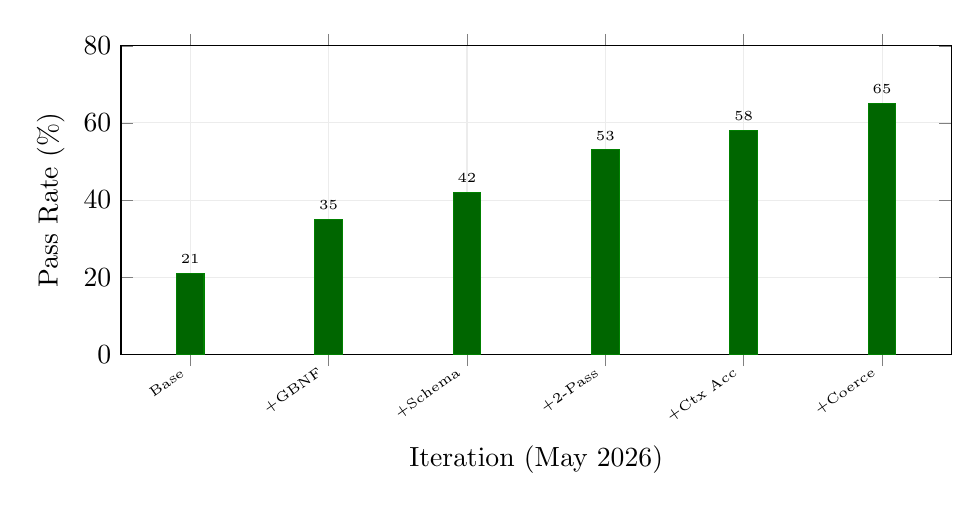
\begin{tikzpicture}
\begin{axis}[
  width=\textwidth,
  height=5.5cm,
  xlabel={Iteration (May 2026)},
  ylabel={Pass Rate (\%)},
  ymin=0, ymax=80,
  xtick={1,2,3,4,5,6},
  xticklabels={Base,+GBNF,+Schema,+2-Pass,+Ctx Acc,+Coerce},
  xticklabel style={font=\tiny, rotate=35, anchor=east},
  ytick={0,20,40,60,80},
  ybar,
  bar width=10pt,
  nodes near coords,
  nodes near coords style={font=\tiny},
  grid=major,
  grid style={gray!15},
  every node near coord/.append style={above, font=\tiny\bfseries},
]
\addplot[fill=green!40!black, draw=green!50!black] coordinates {
  (1, 21) (2, 35) (3, 42) (4, 53) (5, 58) (6, 65)
};
\end{axis}
\end{tikzpicture}
\caption{Phase 1: BFCL-derived pass rates}
\label{fig:arc_phase1}
\end{subfigure}
\hfill
\begin{subfigure}[b]{0.52\textwidth}
\centering
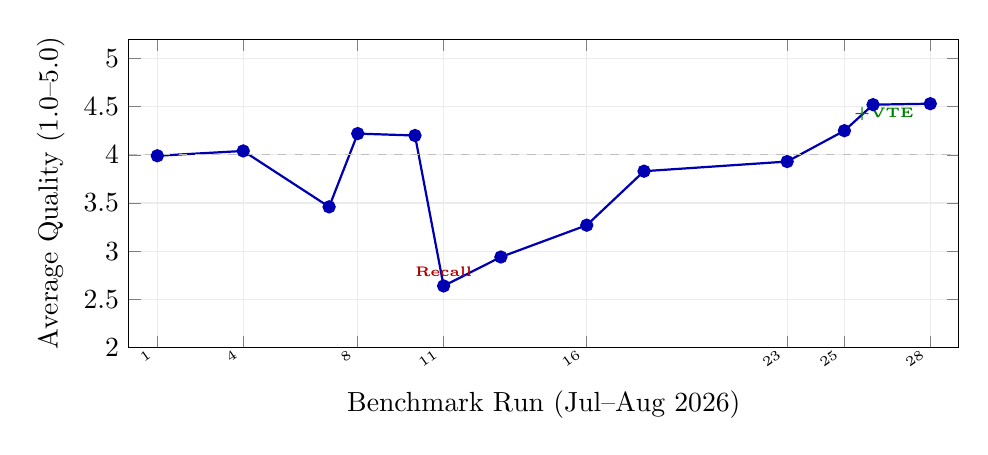
\begin{tikzpicture}
\begin{axis}[
  width=\textwidth,
  height=5.5cm,
  xlabel={Benchmark Run (Jul--Aug 2026)},
  ylabel={Average Quality (1.0--5.0)},
  xmin=0, xmax=29,
  ymin=2.0, ymax=5.2,
  xtick={1,4,8,11,16,23,25,28},
  xticklabel style={font=\tiny, rotate=35, anchor=east},
  ytick={2.0,2.5,3.0,3.5,4.0,4.5,5.0},
  grid=major,
  grid style={gray!15},
  mark options={solid},
]
% Phase 2 quality scores
\addplot[thick, mark=*, blue!70!black, mark size=2pt] coordinates {
  (1, 3.99) (4, 4.04) (7, 3.46) (8, 4.22) (10, 4.20)
  (11, 2.64) (13, 2.94) (16, 3.27) (18, 3.83)
  (23, 3.93) (25, 4.25) (26, 4.52) (28, 4.53)
};

% Annotations
\node[font=\tiny, red!70!black, anchor=south] at (axis cs:11,2.64) {\textbf{Recall}};
\node[font=\tiny, green!50!black, anchor=south west] at (axis cs:25,4.25) {\textbf{+VTE}};

% Reference line
\draw[dashed, gray!50] (axis cs:0,4.0) -- (axis cs:29,4.0);
\end{axis}
\end{tikzpicture}
\caption{Phase 2: LLM-as-judge quality scores}
\label{fig:arc_phase2}
\end{subfigure}
\caption{The full improvement arc across both evaluation phases. \textbf{Left}: Phase 1 (May 2026) tracked binary pass/fail on BFCL-derived parameter extraction tasks, improving from 21\% to 65\% through incremental infrastructure additions. \textbf{Right}: Phase 2 (July--August 2026) used continuous 1.0--5.0 quality scoring on the 25-task suite, showing the regression from the Recall Node overhaul (Run 11, 2.64) and recovery through VTE (Run 28, 4.53). The same 4B model was used throughout both phases.}
\label{fig:improvement_arc}
\end{figure}

Note that Run~1 begins at 3.99---not zero---because the system already incorporated months of Phase~1 learnings (accumulated context architecture, schema coercion, GBNF parameter matching).
The full longitudinal arc spans from Phase~1's 21\% pass rate on basic parameter extraction to Phase~2's 4.53/5.0 on complex multi-step tasks.

We highlight three critical inflection points:

\paragraph{The August 4 regression (4.20 $\to$ 2.64).}
Between Runs 10 and 11, we overhauled the Recall Node architecture to address the ``Synthesis Cliff''---a failure mode where one-shot processing of raw Thought Chain history produced incoherent synthesis at scale.
The new Refinement Pass design (content-aware compaction building a deterministic baseline before agentic refinement) was architecturally sound but initially misconfigured, causing a 1.56-point quality drop---the largest single regression in the evaluation.
Diagnosis took approximately 6 hours across 3 runs (Runs 11--13).

\paragraph{The August 5 recovery (2.64 $\to$ 3.83 in one day).}
Runs 13--18 represent four consecutive improvements on a single day as three subsystems came online simultaneously:
(1) the Spec Compliance Gate began catching missing requirements in code generation tasks;
(2) the Structural Pre-Check's meta-commentary detection filter eliminated degenerate ``As an AI\ldots'' outputs;
and (3) per-node Micro-Skill injection replaced global skill injection, reducing attention dilution in Probe Nodes.
The combined effect recovered 1.19 quality points in four runs.

\paragraph{The August 11--12 final push (3.93 $\to$ 4.53).}
Verified Task Execution completed the quality pipeline: the local model performs full exploration and synthesis, then a cloud model evaluates the output against the original goal and optionally re-synthesizes from the Recall Node's \texttt{refinedContext}.
This added 0.60 quality points by catching and correcting the remaining cases where the local model's synthesis was factually correct but poorly organized or incomplete.

\paragraph{Key takeaway.}
The entire improvement arc---from 21\% pass rate to 4.53/5.0 quality---was achieved without changing the underlying model.
The same 4B-parameter model (Agents-A1-4B, a fine-tuned Qwen-3.5 4B, GGUF Q8\_0 quantization) was used for every run in both phases.
All improvement is attributable to infrastructure: accumulated context, quality gates, content-aware compaction, Phase Runners, and Verified Task Execution.

% ---------------------------------------------------------------------------
\subsection{Quality Results by Category}
\label{sec:eval_category_results}

Table~\ref{tab:category_results} presents the best-achieved average quality scores across the four task categories, along with the number of dedicated benchmark runs per category.

\begin{table}[h]
\centering
\caption{Quality results by task category. ``Dedicated runs'' counts category-specific benchmark iterations beyond the 28 full-suite runs.}
\label{tab:category_results}
\small
\begin{tabular}{@{}lrrll@{}}
\toprule
\textbf{Category} & \textbf{Ded. Runs} & \textbf{Best Avg} & \textbf{Trend} & \textbf{Notes} \\
\midrule
Code generation & 2 & 4.54 & Stable & Strongest---quality gates effective \\
Documentation & 4 & 4.75 & 1.00 $\to$ 4.75 & Dramatic improvement in one day \\
Data analysis & 17 & 3.55 & Volatile & Hardest---SQL reasoning challenging for 4B \\
Web research & 19 & 3.70 & 2.50 $\to$ 3.70 & Phase Runner essential \\
\midrule
\textbf{Full suite} & \textbf{28} & \textbf{4.53} & 3.99 $\to$ 4.53 & All categories combined \\
\bottomrule
\end{tabular}
\end{table}

\paragraph{Per-task distribution (Run 28).}
Of the 25 tasks in Run 28 (the current best at 4.53 average):

\begin{itemize}[leftmargin=*]
\item 16 tasks (64\%) scored \textbf{5.00} --- fully satisfying all requirements
\item 5 tasks (20\%) scored \textbf{4.00--4.99} --- satisfying core requirements with minor gaps
\item 3 tasks (12\%) scored \textbf{3.00--3.99} --- partially satisfying requirements
\item 1 task (4\%) scored \textbf{below 3.00} --- significant gaps
\end{itemize}

The single sub-3.0 task (\texttt{lead\_source\_by\_owner}, scoring 1.75) and the three tasks scoring 3.00--3.99 are all data analysis tasks requiring SQL reasoning against the cached dataset.
All code generation and documentation tasks scored $\geq$4.00.
This distribution reveals a clear capability boundary: the 4B model handles code generation, exploration, and synthesis reliably, but struggles with complex SQL query composition---a finding consistent with the data analysis category's overall lower scores.

% ---------------------------------------------------------------------------
\subsection{Cost Analysis}
\label{sec:eval_cost}

Table~\ref{tab:cost_analysis} presents the token consumption and cost breakdown for Run 28.

\begin{table}[h]
\centering
\caption{Token consumption and cost analysis for Run 28 (25 tasks, cooperative mode).}
\label{tab:cost_analysis}
\small
\begin{tabular}{@{}lr@{}}
\toprule
\textbf{Metric} & \textbf{Value} \\
\midrule
Total cloud tokens & 243,911 \\
\quad Prompt tokens & 204,547 \\
\quad Completion tokens & 39,364 \\
Total local tokens & 1,661,896 \\
Total estimated cost & \$2.57 \\
Average cost per task & \$0.10 \\
Cost per quality point & \$0.02 / quality-point / task \\
\midrule
Cloud inference calls & 67 (across 25 tasks) \\
Local inference calls & 412 (across 25 tasks) \\
Cloud:Local inference ratio & 1:6.1 \\
\bottomrule
\end{tabular}
\end{table}

The cost structure confirms the routing hypothesis (Section~\ref{sec:cost_arbitrage}): 86\% of inference calls (412 of 479 total) are handled locally at zero marginal cost.
Cloud inference is reserved for Complexity Tier routing (T2 planning), Confidence Tier escalation (parameter extraction failures), and Verified Task Execution (terminal output verification).
The average task requires 2.7 cloud inference calls and 16.5 local inference calls.

% ---------------------------------------------------------------------------
\subsection{Latency Profile}
\label{sec:eval_latency}

Wall-clock execution times ranged from 22.9 seconds (\texttt{create\_hello\_handler}, a simple code generation task with 0 tool calls) to 23.9 minutes (\texttt{comprehensive\_readme}, a full-codebase documentation task with 25 tool calls).
Table~\ref{tab:latency} shows representative tasks across the latency spectrum.

\begin{table}[h]
\centering
\caption{Representative wall-clock execution times from Run 28.}
\label{tab:latency}
\small
\begin{tabular}{@{}llrrrr@{}}
\toprule
\textbf{Task} & \textbf{Category} & \textbf{Wall (s)} & \textbf{Tools} & \textbf{Local Tok} & \textbf{Quality} \\
\midrule
create\_hello\_handler & Codegen & 23 & 0 & 1,090 & 5.00 \\
update\_add\_method & Codegen & 27 & 0 & 2,001 & 5.00 \\
create\_config\_parser & Codegen & 67 & 0 & 3,556 & 5.00 \\
security\_advisory\_lookup & Research & 98 & 4 & 16,848 & 5.00 \\
lead\_count\_by\_country & Data Anal. & 238 & 7 & 47,181 & 4.25 \\
internal\_architecture & Exploration & 237 & 4 & 106,129 & 5.00 \\
inference\_module\_docs & Exploration & 417 & 6 & 159,473 & 4.50 \\
cache\_function\_index & Exploration & 513 & 10 & 306,760 & 5.00 \\
comprehensive\_readme & Exploration & 1,432 & 25 & 698,165 & 5.00 \\
\bottomrule
\end{tabular}
\end{table}

Latency correlates strongly with local token consumption ($r = 0.98$) and tool call count ($r = 0.91$), not with cloud token usage ($r = 0.34$).
This confirms that the bottleneck is local inference throughput and exploration depth, not cloud API latency---an expected consequence of the local-first architecture.

% ---------------------------------------------------------------------------
\subsection{Category-Specific Analysis}
\label{sec:eval_category_deep}

\subsubsection{Data Analysis: The Hardest Category}

Data analysis tasks achieved a best average of 3.55 across 17 dedicated runs---the lowest of any category.
The core challenge is SQL query composition: the 4B model must translate natural language analytical questions into valid SQL against an unfamiliar schema, then interpret the results.

Three mechanisms improved data analysis quality during the evaluation period:
(1) the \emph{Deterministic Query Path}, which bypasses the Thought Chain for high-confidence queries (Query Confidence $\geq$0.70) using regex-based intent extraction and direct SQL assembly;
(2) the \emph{Aggregate Row-Count Validation}, which catches malformed GROUP BY clauses by comparing aggregate output against known table cardinality;
and (3) the \emph{SQL Cache Store}, which materializes tabular data into ephemeral SQLite tables rather than relying on raw text in the context window.

Despite these improvements, data analysis remains the weakest category.
The primary failure mode is multi-step analytical reasoning: tasks requiring sequential queries (e.g., ``find the lead owner with the most leads, then break down their leads by sector'') often fail at the second step because the model loses track of intermediate results.

\subsubsection{Web Research: Phase Runner as the Unlock}

Web research tasks improved from 2.50 to 3.70 across 19 dedicated runs.
The critical inflection point was the introduction of the Phase Runner, which replaced the flat Thought Chain with a structured 5-phase pipeline: Search $\to$ Rank $\to$ Deep-Read $\to$ Cross-Ref $\to$ Synthesize.

Under the flat Thought Chain, the 4B model consistently hit a quality ceiling around 2.5---it would search, read one or two results, and immediately attempt synthesis without cross-referencing sources.
The Phase Runner's scoped tool budgets (Search phase: only \texttt{web\_search}; Deep-Read phase: only \texttt{web\_browse}) forced the model through a disciplined exploration sequence, and the per-phase step budgets prevented premature synthesis.

\subsubsection{Documentation: From 1.00 to 4.75 in One Day}

Documentation generation showed the most dramatic improvement: 4 dedicated runs on August 7 progressed from 1.00 to 1.25 to 0.00 (a crash) to 4.75.
The crash in Run 3 exposed a bug in the MapReduceSynthesis path for large codebases, where the reduce phase received empty chunk summaries.
After fixing the reduce-phase input assembly, the system achieved 4.75---its highest category score---by correctly routing between Direct Synthesis (single-shot inference for small codebases) and MapReduceSynthesis (chunked summarization for large ones).


% ============================================================================
\section{Related Work}
\label{sec:related_work}
% ============================================================================

\paragraph{Agent architectures and reasoning.}
ReAct~\cite{react2023} introduced the interleaved reasoning-and-acting paradigm that most agent frameworks now follow.
AutoGen~\cite{autogen2023}, CrewAI~\cite{crewai2024}, and LangChain/LangGraph~\cite{langchain2023} provide orchestration layers built on this paradigm.
All three default to frontier models for every inference call and implement agent loops (conversational turns or cyclic graph execution) rather than compiled DAGs.
LangGraph's ``cyclic graph'' model is closest to \textsc{tzro}'s DAG approach, but it permits arbitrary cycles and relies on the frontier model to decide loop termination---making execution non-deterministic and cost unbounded.
\textsc{tzro}'s Kahn-compiled DAGs are acyclic by construction; dynamism is contained inside Probe Nodes (bounded step budgets) rather than in the graph topology.

Reflexion~\cite{reflexion2023} introduces verbal reinforcement learning, where an agent reflects on failures and generates textual feedback for future attempts.
\textsc{tzro}'s Corrective Micro-Skills serve a related function---encoding failure-correction pairs for future injection---but operate at the node level rather than the task level, and persist across tasks rather than within a single retry loop.

DSPy~\cite{dspy2023} compiles declarative LM programs into optimized prompts through automatic few-shot example selection.
\textsc{tzro}'s Plan Templates and Micro-Skill injection are conceptually similar (scaffolding the model's behavior without weight updates), but operate at the execution graph level rather than the prompt optimization level.
DSPy optimizes individual LM calls; \textsc{tzro} optimizes multi-step workflows.

\paragraph{Small model capabilities.}
Phi-3~\cite{phi3technical2024} and Llama 3~\cite{llama3herd2024} demonstrate that models with 1--8B parameters can match larger models on specific benchmarks.
Mixtral~\cite{mixtral2024} shows that sparse mixture-of-experts architectures achieve strong performance with fewer active parameters per token.
Our work extends these findings from isolated benchmarks to sustained agentic workflows, showing that architectural support (task decomposition, quality gates, scoped skill injection) enables reliable agentic execution at the 4B scale.
Our worker model, Agents-A1-4B~\cite{agentsa1_2025}, is a fine-tune of Qwen-3.5 4B optimized for agentic tool-use; our Edit Loop and Preservation Assertion mechanisms address the remaining failure modes (symbol dropping, full-file degeneration) specific to agentic code generation where the model must surgically modify existing files rather than generate from scratch.

\paragraph{Model routing and cost optimization.}
RouteLLM~\cite{routellm2024} trains a router to direct queries to strong or weak models based on predicted difficulty, using human preference data for training.
FrugalGPT~\cite{frugalgpt2023} cascades through models of increasing capability.
Both optimize individual inference calls.
\textsc{tzro}'s two-tier routing differs in three ways: (1) it operates at both the task level (Complexity Tier) and the per-node level (Confidence Tier), rather than per-call; (2) routing decisions are based on structural task analysis (does this require graph-level planning?) rather than predicted difficulty; and (3) failed local routing produces Corrective Micro-Skills that progressively reduce future escalation rates---the routing policy self-improves with use.
Speculative decoding~\cite{speculative2023} achieves inference speedup by using a small draft model to propose tokens that a large model verifies.
\textsc{tzro}'s Worker/Router architecture is architecturally analogous (a larger model reasons, a smaller model structures), but operates at the semantic level (reasoning vs.\ action extraction) rather than the token level.

\paragraph{Constrained decoding and structured output.}
GBNF grammars~\cite{ggerganov_llamacpp} and Outlines~\cite{outlines2024} enable structured output from language models by constraining the decoding process.
\textsc{tzro} uses GBNF extensively but contributes two design insights.
First, the two-pass separation of unconstrained reasoning from constrained extraction achieves higher reliability than constraining the generation itself---the single-pass approach failed approximately 90\% of the time on action tag emission.
Second, deep GBNF schemas (nested JSON with many required fields) degrade inference speed 2--5$\times$; \textsc{tzro}'s Semantic Validator replaces deep grammars with shallow structural constraints plus post-hoc coercion, trading grammar guarantees for speed without measurable accuracy loss.

\paragraph{Durable execution.}
Temporal~\cite{temporal2022} and Prefect provide durable workflow execution for conventional software with deterministic retries and state recovery.
\textsc{tzro} applies these principles to LLM workflows, but faces challenges unique to non-deterministic nodes: (1) replaying a crashed node produces different output than the original execution, requiring content-aware checkpointing rather than input replay; (2) the system must distinguish between node failures (retry) and model quality failures (escalate); and (3) two-level durability (DAG-level and probe-step-level) is needed because Probe Nodes contain their own multi-step execution.

\paragraph{Tool-use and function calling.}
Toolformer~\cite{toolformer2023} fine-tunes models to learn tool-use end-to-end.
ToolLLM~\cite{toolllm2023} provides a framework for training and evaluating tool-use across 16,000+ APIs.
The BFCL~\cite{bfcl2024} and Gorilla~\cite{gorilla2023} evaluate tool-use in isolation.
Our Phase 1 evaluation adapted BFCL methodology; the key finding was that isolated tool-call accuracy does not predict end-to-end task quality.
The Confidence Tier and Corrective Micro-Skills address this gap by providing runtime adaptation rather than training-time optimization.
SWE-agent~\cite{sweagent2024} and SWE-bench~\cite{swebench2024} evaluate end-to-end software engineering capabilities but use frontier models exclusively.
\textsc{tzro}'s code generation quality gates (Compilation Gate, Spec Compliance Gate, Preservation Assertion) address the same problem space at the 4B scale.

\paragraph{Retrieval-augmented generation.}
Standard RAG~\cite{rag2020} retrieves documents from a static corpus to provide generation context.
\textsc{tzro}'s Recall Node performs a related function but differs in two important ways: it operates on \emph{execution traces} rather than document corpora (the ``documents'' are tool outputs from prior exploration steps), and it uses content-type-aware compaction (code skeletons, fact extraction, tabular sampling) rather than uniform chunking.
The Symbol Anchor Check (verifying that referenced code symbols exist in the AST-extracted index) provides a form of retrieval-grounded verification absent from standard RAG pipelines.

% ============================================================================
\section{Discussion and Lessons Learned}
\label{sec:discussion}
% ============================================================================

Four high-level findings emerged from building and evaluating \textsc{tzro}:

\paragraph{1.\ Infrastructure dominates parameters.}
The quality improvement from 2.64 to 4.53 was achieved with \emph{zero model changes}---the same 4B GGUF weights throughout.
Every improvement came from infrastructure: better compaction, structured phases, binding splices, validation gates.
This suggests that the current discourse around model scaling may underweight the contribution of execution infrastructure.

\paragraph{2.\ Nine compensatory mechanisms is the wrong abstraction.}
By the time Verified Task Execution was introduced, the system contained nine separate mechanisms compensating for local model failures.
Each mechanism was individually justified, but the interaction space was exponential---tuning one mechanism's thresholds caused regressions in another.
The correct abstraction was a single verification gate that accepts or rejects, with all prior mechanisms reframed as ``maximize the accept rate'' rather than ``compensate for bad output.''

\paragraph{3.\ Domain language prevents architectural drift.}
The formal vocabulary with anti-terms (\emph{Avoid: pipeline, automation track} for the Kahn Compiler) proved essential as the system grew to 76 ADRs.
AI contributors in particular benefit from anti-terms: without them, a model generating code or documentation will use natural synonyms that carry incorrect architectural connotations, gradually blurring the boundaries between concepts.

\paragraph{4.\ Evaluation methodology must evolve with the system.}
Phase 1 (BFCL-derived parameter extraction) became inadequate when end-to-end quality, not individual tool calls, became the bottleneck.
Phase 2 (LLM-as-judge quality scoring) revealed new blind spots (the docgen inter-rater gap: 4.25 cloud judge vs.\ 2.65 local model cross-verification).
A longitudinal evaluation must treat its own methodology as a variable, not a constant.

\subsection{Limitations}
\label{sec:limitations}

Several significant limitations constrain the generality of our findings:

\paragraph{Data analysis remains weak.}
The 4B model achieves only 3.55/5.0 on data analysis tasks---the lowest category score by a significant margin.
SQL query composition, particularly multi-step analytical reasoning where intermediate results must carry between queries, consistently exceeds the model's effective reasoning capacity.
The Deterministic Query Path handles simple queries well, but complex analytical questions (e.g., sequential aggregation with filtering) require frontier-level reasoning.
This represents a genuine capability boundary, not a decomposition problem.

\paragraph{LLM-as-judge limitations and inter-rater disagreement.}
Our primary quality scoring relies on a cloud LLM-as-judge (Gemini 3.5 Flash).
Cross-verification using the local 4B model as an independent second judge revealed significant inter-rater disagreement: on documentation tasks, the cloud judge scored 4.25/5.0 while the local model scored 2.65/5.0---a 38\% gap.
Neither score represents human ground truth.
The cloud judge appears to reward structural formatting and coherent prose without adequately verifying factual accuracy.
The local model, conversely, may be overly sensitive to outputs that differ from its own generation patterns.
Without a human evaluation baseline, we cannot determine which judge is more accurate, only that the disagreement exists and is category-dependent.
The Symbol Anchor Check partially addresses this for code-related outputs by grounding verification in the AST, but no equivalent mechanism exists for web research or general knowledge synthesis.
Future work should incorporate human evaluation on a representative subset to calibrate both judges.

\paragraph{Single-model evaluation.}
All results are from a single model: Agents-A1-4B (a fine-tune of Qwen-3.5 4B, GGUF Q8\_0).
While this strengthens the ``infrastructure dominates parameters'' claim (all improvement comes from infrastructure, not model changes), it limits generalizability.
The techniques described here may produce different improvement curves on other model families, particularly those with different attention patterns or instruction-following characteristics.

\paragraph{Single-evaluator benchmark.}
The 25-task benchmark suite was designed by a single developer for a specific codebase.
The task distribution may not represent the broader space of agentic workloads.
In particular, the suite lacks tasks requiring multi-turn user interaction, real-time system integration, or adversarial inputs.

\paragraph{Privacy-quality tradeoff.}
The \texttt{strict-local} privacy mode disables Verified Task Execution, accepting higher output variance in exchange for complete data locality.
We have not quantified the quality degradation under strict-local mode, though the 4.20 $\to$ 4.53 improvement attributable to VTE (Runs 10 vs.\ 28) provides an upper bound estimate.

\paragraph{Hardware specificity.}
All experiments ran on a single Apple Silicon machine with 24GB unified memory.
Inference throughput, thermal throttling behavior, and memory pressure characteristics are specific to this hardware class.
The system's performance on Linux servers with discrete GPUs, or on machines with less memory (requiring smaller quantizations), remains unevaluated.

% ============================================================================
\section{Conclusion}
\label{sec:conclusion}
% ============================================================================

We presented \textsc{tzro}, a durable execution engine that makes 4B-parameter models reliable agents through architectural support rather than model scaling.
The system compiles natural language prompts into checkpointed DAGs, routes 86\% of inference calls to a local model at zero marginal cost, and achieves 4.53/5.0 average quality on a diverse 25-task benchmark suite.

The key insight is that most agentic work is \emph{routing}---tool selection, parameter extraction, navigation---not \emph{reasoning}.
When the orchestration harness decomposes work into properly-scoped routing decisions, a 4B model executes reliably.
The narrow residual cases requiring frontier reasoning are handled through surgical cloud escalation, keeping total costs at \$0.10/task.

The system's architecture---Probe Nodes for bounded exploration, Phase Runners for structured execution, content-aware compaction for context management, Verified Task Execution for quality assurance, and per-node Micro-Skill injection for self-improvement---represents a toolkit of techniques for making small models capable agents.
We release the full system, benchmark suite, and 76 Architecture Decision Records as open source to enable reproduction and extension of these results.


\bibliographystyle{plain}
\bibliography{references}

% ============================================================================
% APPENDICES
% ============================================================================
\appendix

\section{Domain Glossary}
\label{app:glossary}

Table~\ref{tab:glossary} presents a selected subset of the $\sim$120-term formal vocabulary maintained in the project's \texttt{CONTEXT.md}.
Each term includes an anti-term list (synonyms that are explicitly prohibited) to prevent architectural drift.

\begin{table}[h]
\centering
\small
\begin{tabular}{@{}llp{5.5cm}@{}}
\toprule
\textbf{Term} & \textbf{Anti-terms} & \textbf{Definition} \\
\midrule
Kahn Compiler & pipeline, automation track & Topological sorter producing parallel execution layers from Abstract Graphs \\
Probe Node & scanner, crawler & Bounded autonomous exploration node running a Thought Chain internally \\
Phase Runner & pipeline, Thought Chain & State machine executing structured phase sequences within a single DAG node \\
Complexity Tier & difficulty score & Task-level routing: T0 Direct, T1 Planned, T2 Supervised \\
Confidence Tier & difficulty score & Per-node pre-flight self-assessment for parameter extraction \\
Code Skeleton & AST extraction & Deterministic compaction preserving signatures and comments \\
Execution Envelope & response, result & Structured container wrapping task output with metadata and verification \\
\bottomrule
\end{tabular}
\caption{Selected domain glossary entries with anti-terms.}
\label{tab:glossary}
\end{table}

\section{Architecture Decision Record Index}
\label{app:adr_index}

The project maintains 76 Architecture Decision Records (ADRs) documenting every significant design decision.
Key ADRs referenced in this paper include:

\begin{table}[h]
\centering
\small
\begin{tabular}{@{}rl@{}}
\toprule
\textbf{ADR} & \textbf{Title} \\
\midrule
0010 & Local-default / cloud-exception model routing \\
0019 & Probe Node and Thought Chain execution \\
0020 & Confidence Tier and Corrective Micro-Skills \\
0022 & Background Agent abstraction and Observer refactor \\
0030 & Proactive Binding Splice for deterministic resolutions \\
0047 & AST-based Symbol Extraction for Probe Nodes \\
0048 & Plan Template Selection and Mutation \\
0055 & Structured Execution Envelope \\
0062 & Execution Pipeline Acceleration (Substrate Modes) \\
0064 & Two-Pass Extraction and Recall Inversion \\
0066 & ModelTarget Routing and Synthesis Validation Gate \\
0067 & Verified Task Execution \\
0073 & PhaseRunner Tool Hooks \\
\bottomrule
\end{tabular}
\caption{Selected ADRs referenced in this paper. The full index is available in the repository.}
\end{table}

\section{Benchmark Run Index}
\label{app:benchmark_index}

The evaluation spans 70+ surviving benchmark runs.
Phase 1 runs (May--June 2026, BFCL-derived) are partially lost due to storage cleanup; their results are preserved in wiki post-mortem documents.
Phase 2 runs (July--August 2026, quality-scored) are fully preserved in the repository under \texttt{.scratch/benchmark/}.
Table~\ref{tab:run_index} lists the milestone runs.

\begin{table}[h]
\centering
\small
\begin{tabular}{@{}rllr@{}}
\toprule
\textbf{Run} & \textbf{Date} & \textbf{Key Change} & \textbf{Avg Quality} \\
\midrule
1 & Jul 27 & Baseline (flat Thought Chain) & 3.99 \\
4 & Jul 27 & Minor tuning & 4.04 \\
7 & Jul 28 & Regression from refactor & 3.46 \\
8 & Jul 29 & Recovery + context improvements & 4.22 \\
10 & Jul 29 & Stabilization & 4.20 \\
\midrule
11 & Aug 4 & Recall Node architecture overhaul & 2.64 \\
13 & Aug 4 & Incremental recovery & 2.94 \\
16 & Aug 5 & Quality gates coming online & 3.27 \\
18 & Aug 5 & Recall Node Refinement Pass & 3.83 \\
\midrule
23 & Aug 7 & Phase Runner stabilization & 3.93 \\
25 & Aug 11 & Verified Task Execution deployed & 4.25 \\
26 & Aug 12 & Final tuning pass & 4.52 \\
28 & Aug 12 & Current best & 4.53 \\
\bottomrule
\end{tabular}
\caption{Complete Phase 2 benchmark run index. All runs use the same 4B model; only infrastructure changed between runs.}
\label{tab:run_index}
\end{table}

\section{System Configuration}
\label{app:system_config}

All experiments were conducted on a single Apple MacBook Pro with the following configuration:

\begin{itemize}[leftmargin=*]
\item \textbf{Hardware}: Apple M-series processor, 24GB unified memory
\item \textbf{Worker model}: Agents-A1-4B (fine-tune of Qwen-3.5 4B; Q8\_0 GGUF quantization), running via llama.cpp server with batch size 2048, parallel slots 2. Available at \url{https://huggingface.co/InternScience/Agents-A1-4B}.
\item \textbf{Router model}: Qwen-3.5 0.6B Instruct (Q8\_0 GGUF quantization), running as speculative decoding draft with n-gram simple, draft-n-max 16
\item \textbf{Cloud model}: Google Gemini 3.5 Flash (via API, used for T0/T2 routing and Verified Task Execution)
\item \textbf{Embedding model}: Nomic Embed v1.5 (ONNX, runs locally for semantic retrieval)
\item \textbf{Database}: SQLite 3 (single file, WAL mode) for all persistence
\end{itemize}

\end{document}
